The second run period of the LHC starting in 2015 at a centre of mass energy of $\sqrt{s} = 13$\tev provides the excellent opportunity to further investigate the question, if supersymmetry is realised in nature at the \tev scale. As discussed in Section~\ref{sec:susy_status}, the current limits exclude stop quarks with masses up to around 750\gev for LSP masses below 100\gev in case of direct stop production. Since in case of natural supersymmetry the stop quark mass is expected to not exceed the 1\tev significantly, it is thus of particular interest to probe the stop mass range $\ge 750$\gev for light LSPs. \\
The targeted process of this analysis is illustrated in a diagram in Fig.~\ref{fig:T2tt} below. \\ 
\begin{figure}[!h]
  \centering
  \begin{tabular}{c}
                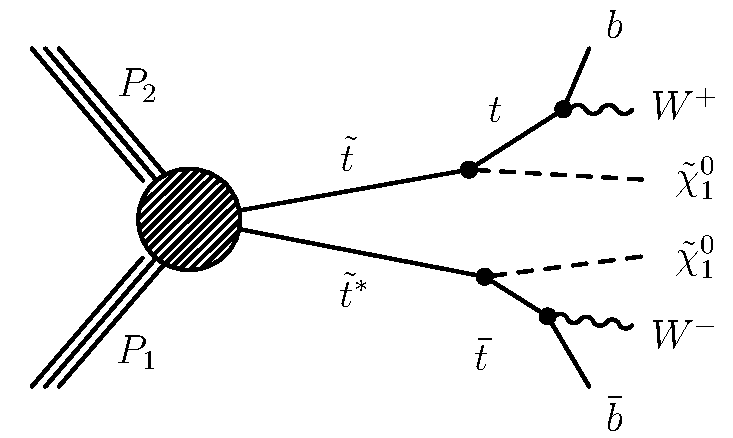
\includegraphics[width=0.49\textwidth]{figures/T2tt.pdf} 
  \end{tabular}
  \caption{Schematic diagram of the direct pair production of stop quarks in pp collisions with subsequent decay into a top quark and the LSP. Taken from~\cite{bib:CMS:PhysicsResultsSUS}. }
  \label{fig:T2tt}
\end{figure}
   
Here, the pair production of top squarks is shown with subsequent decay into a top quark and the LSP. Since the top quark decays into a b quark and a W boson, the expected final state signature further depends on the decay modes of the W boson. In this analysis, only final states with fully hadronic top decays are considered. Consequently, this analysis targets a jet final state accompanied by missing transverse energy caused by the LSPs. As discussed in Section~\ref{subsec:susy_collider}, background contributions from the SM to such signatures arise mainly from QCD multijet events, \WJets, \ZJets and \ttbar events. \\
In this Chapter, various analysis strategies for a search for top squarks at $\sqrt{s} = 13$\tev are discussed and compared in order to address mass scenarios with large mass differences between the stop quark mass and the LSP. Furthermore, the performance of studied selections is compared to the existing all-hadronic stop search performed by the CMS experiment at $\sqrt{s} = 8$\tev which is published in~\cite{CMS-PAS-SUS-13-015}. In addition, it is interesting to study, if selections that are found to be suited for direct stop production are also sensitive to the gluino-mediated production of third generation quarks. \\

\section{Data samples}
\label{sec:stop_samples}

\section{Sensitivity of a Basic Selection using \HT and \met}
\label{sec:stop_baseline}
The targeted signature of the direct pair production of stops in the all-hadronic channel is based on jets and missing transverse momentum similar to the search presented in Chapter~\ref{chap:RA2}. Thus, a very similar baseline selection is employed as a basis for further studies. An advantage of such a choice is that a synchronized baseline selection would allow to utilize the same triggers to collect the data. The applied selections are
\begin{itemize}
 \item{Background contributions arising from \ttbar and \WJets events are reduced by rejecting events containing isolated electrons or muons with $\pt > 10$\gev and $|\eta| < 2.5$. These are required to have a good quality track that can be associated with the primary interaction vertex~\cite{CMS-PAS-EGM-10-004, CMS-PAS-MUO-10-002}. The isolation is given as the scalar sum of transverse momenta of PF particles (except for the lepton itself) within a cone of width $\Delta R = 0.3$ for the electron and $\Delta R = 0.4$ for the muon, respectively. This is required to be less than 20\% of the transverse momentum of the electron and less than 15\% of the transverse momentum of the muon.}
 \item{The number of jets (\NJets) is required to be $\ge 3$. \NJets is defined as the number of jets with $\pt > 50$\gev and $|\eta| < 2.5$. This requirement is imposed in order to select multijet events as expected from the two top quarks.}
 \item{The scalar sum of jet momenta (\HT) is required to be $\ge 500$\gev with 
\begin{equation*}
\HT = \sum_{\mathrm{jets}} \pt 
\end{equation*}
for all jets that have $\pt > 50$\gev and $|\eta| < 2.5$. This condition selects events with a large visible energy in the event indicating a high energy scale of the hard interaction.}   
 \item{The missing transverse energy \met calculated from the PF candidates is required to be $\ge 200$\gev. This selection reduces contributions from standard model processes where missing transverse momentum is expected to be small. Especially, QCD multijet background is suppressed. } 
 \item{In order to suppress events where missing transverse energy is mainly arising from jet mismeasurements, as for QCD multijet events, it is required that \met is not aligned with the leading three jets. Thus, events with
\begin{equation*}
\Delta \phi(\mathrm{jet}_n, \met) > 0.5 \;\; \mathrm{for} \;\; n = 1,2 \;\; \mathrm{and} \;\; \Delta \phi(\mathrm{jet}_3, \met) > 0.3
\end{equation*} 
are selected. The value of 0.5 is chosen according to the jet size parameter. However, this is reduced in case of the third jet in order to retain signal efficiency. }
\end{itemize}
Since only simulated events are used, no dedicated event cleaning filters are applied as it is necessary for data (cf. Sec~\ref{subsec:RA2_cleaning}). The selection described here is denoted \textit{baseline} selection in the following. In Tab.~\ref{tab:stop_baseline_cutflow} the event yields of background and two signal processes obtained from simulation normalized to an integrated luminosity of 19.5\fbinv are shown after various requirements together with the statistical uncertainty. It is visible that the \met and $\Delta \phi$ requirement reject most of the background events. After the baseline selection the background is composed quite equally of all four SM processes. Furthermore, in Fig.~\ref{fig:stop_baseline}, the obtained spectra of \HT, \met and \NJets after applying the baseline selection are shown for the SM backgrounds and two selected signal points. The signal points represent mass values of 600\gev and 1100\gev for the stop mass while the LSP mass is in both cases 50\gev. These two signal points illustrate the difference in the kinematic properties of events for low and high stop masses. Typically, the \HT and \met spectrum get harder for higher stop masses while the shape of the \NJets spectrum stays nearly unchanged. \\
\begin{table}[!t]
\fontsize{9 pt}{1.2 em}
\selectfont
\centering
\caption{Event yields and cut flow from MC simulated samples after various requirements described in the text. All numbers are scaled to 19.5\fbinv. Only statistical uncertainties are shown in the table. The signal points are labeled as (X, Y) where X is the top squark mass and Y is the LSP mass.}
\makebox[\linewidth]{
\begin{tabular}{cccccc}
\multicolumn{6}{c}{} \\
  \toprule
   Process & e/$\mu$ veto & jet counting & \HT & \met & $\Delta \phi$  \\
  \midrule
   \ttbar & 10712200 $\pm$ 9170 & 6431190 $\pm$ 7105 & 1274570 $\pm$ 3163 & 34616.8 $\pm$ 521.3 & 16444.9 $\pm$ 359.3 \\
   \WJets & 713523000 $\pm$ 159183000 & 1522960 $\pm$ 20432.5 & 196599 $\pm$ 1259.5 & 25104.5 $\pm$ 295.7 & 12520 $\pm$ 211.6 \\
   \ZJets & 203002000 $\pm$ 408457 & 364126 $\pm$ 4090.1 & 60043.1 $\pm$ 212.4 & 16245.7 $\pm$ 104.9 & 11858.0 $\pm$ 91.1 \\
   QCD multijet & $4.96 \cdot 10^{11}$ $\pm$ $6.89 \cdot 10^{8}$ & $1.01 \cdot 10^{10}$ $\pm$ $8.58 \cdot 10^7$ & $4.43 \cdot 1^{8}$ $\pm$ $3.54 \cdot 10^{6}$ & 109456 $\pm$ 19090 & 20013 $\pm$ 18085 \\
\midrule
   Signal (600, 50) & 2252.7 $\pm$ 8.8 & 1994.7 $\pm$ 8.3 & 1478.3 $\pm$ 7.1 & 1157.9 $\pm$ 6.3 & 1013.1 $\pm$ 5.9 \\
   Signal (1100, 50) & 42.9 $\pm$ 0.2 & 37.3 $\pm$ 0.2 & 36.0 $\pm$ 0.1 & 33.2 $\pm$ 0.1 & 29.2 $\pm$ 0.1 \\
  \bottomrule
\end{tabular}}
\label{tab:stop_baseline_cutflow}
\end{table}    

\begin{figure}[!t]
  \centering
  % \makebox[\linewidth]{
  \begin{minipage}[c]{1.\textwidth}
    \begin{center}
      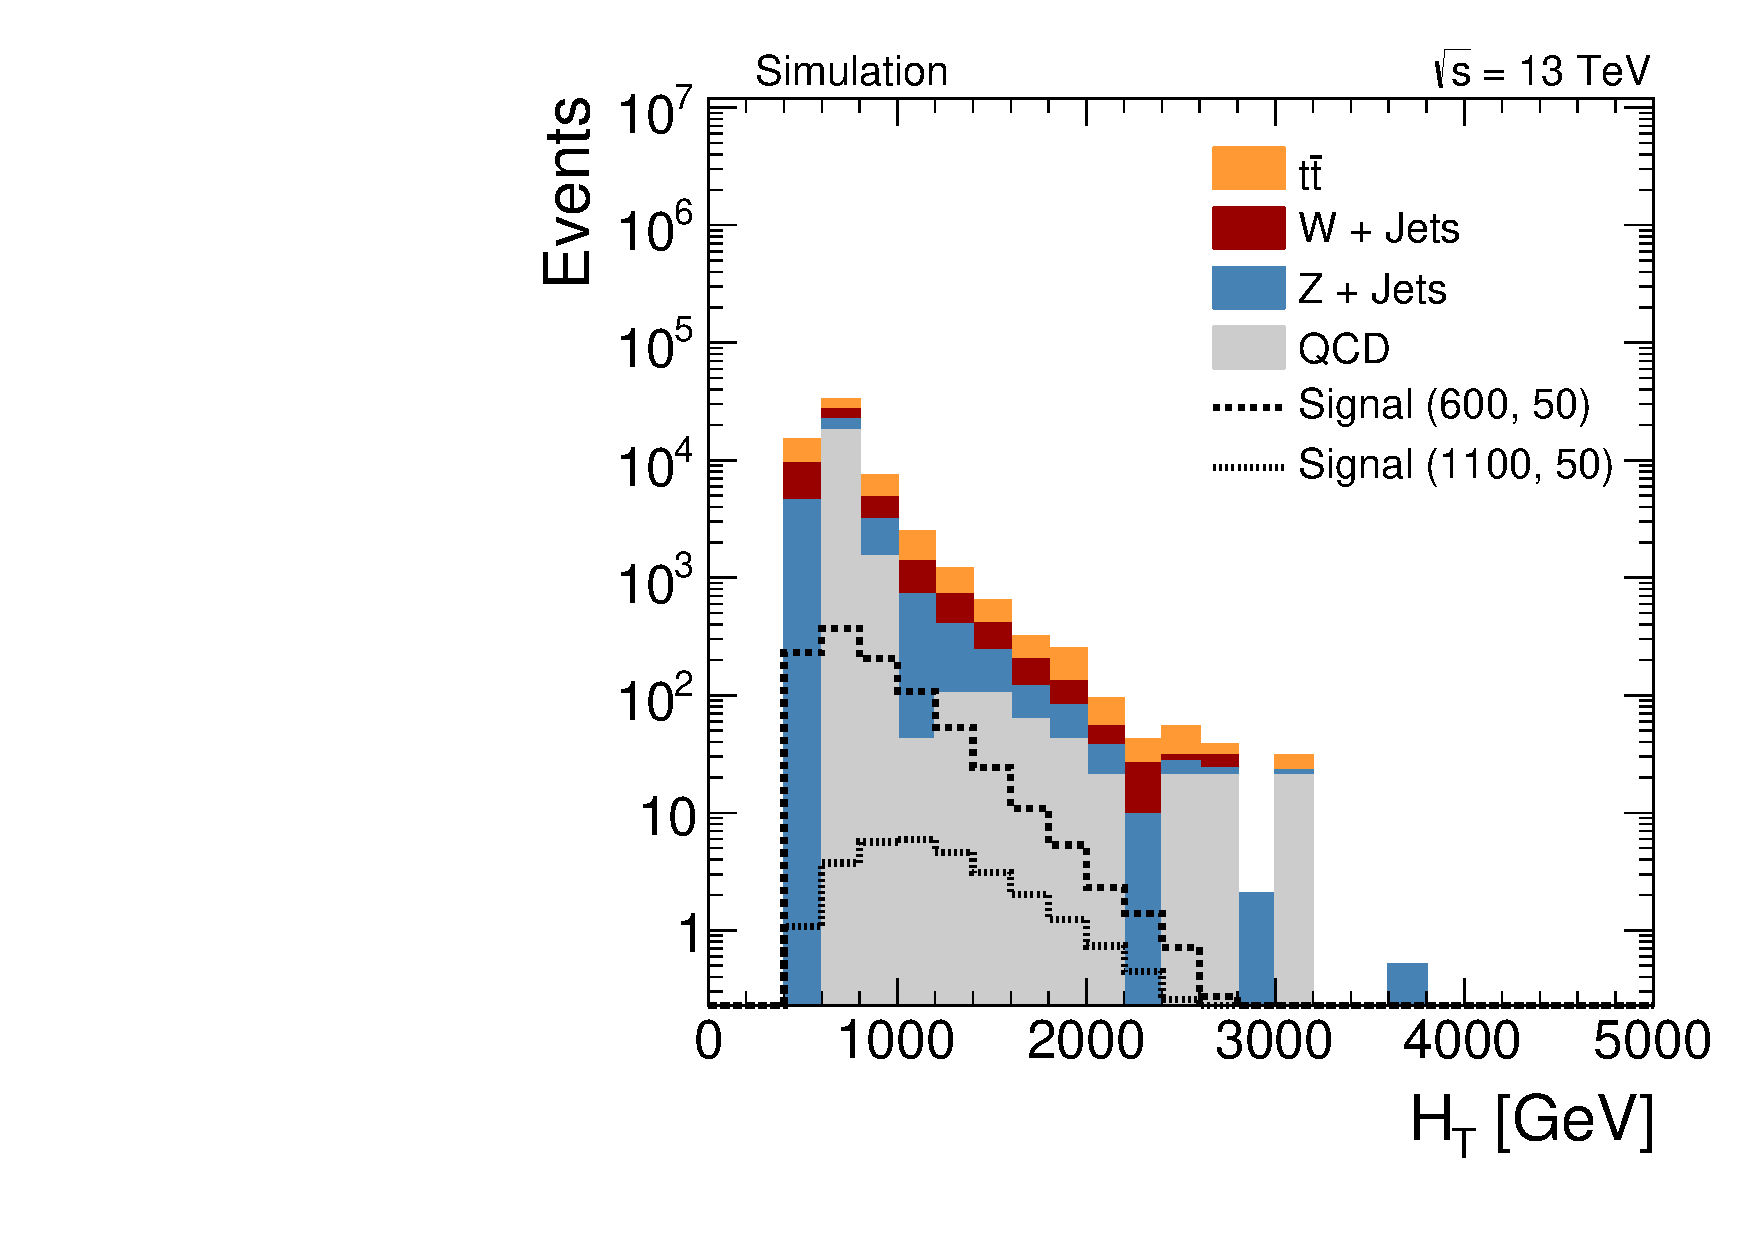
\includegraphics[width=0.49\textwidth]{figures/Stop_DeltaPhiSelection_HThad.pdf}  
      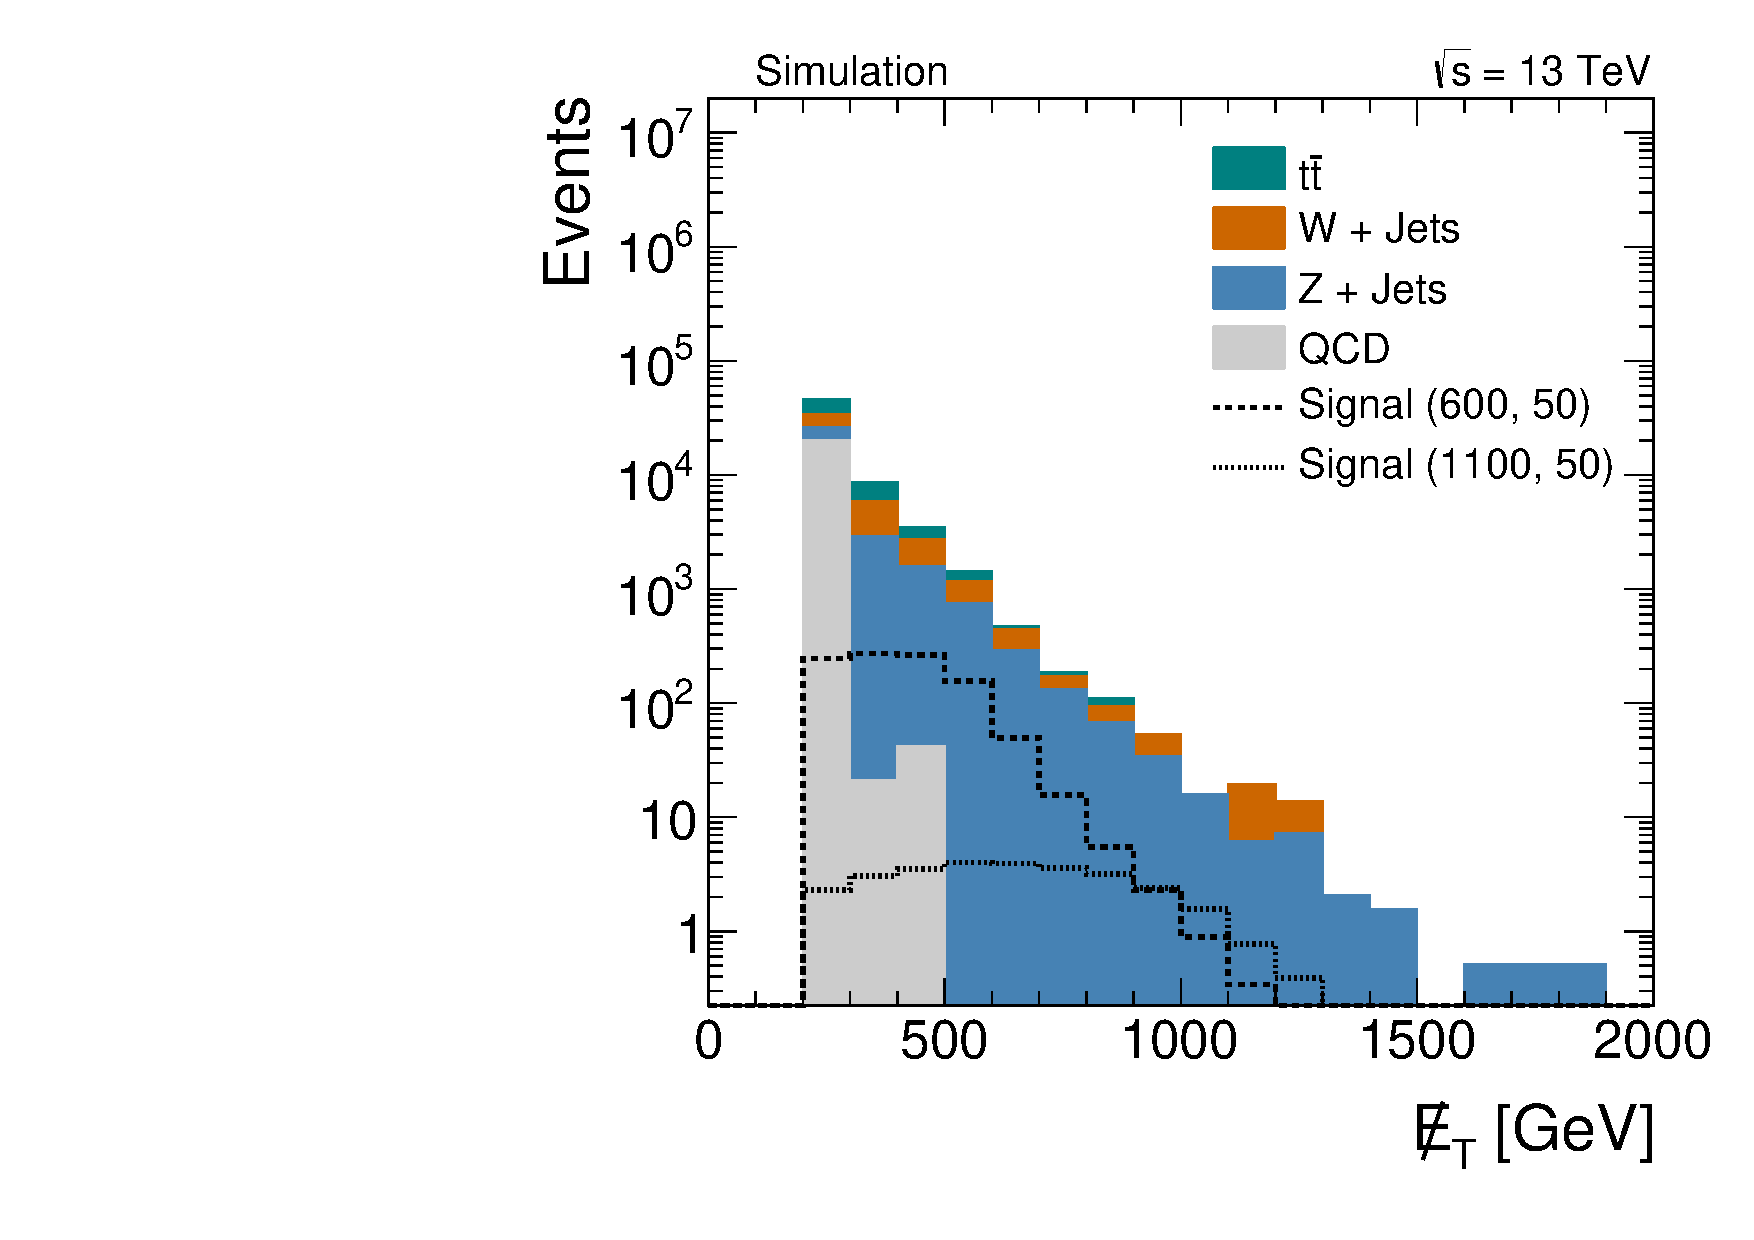
\includegraphics[width=0.49\textwidth]{figures/Stop_DeltaPhiSelection_MET.pdf} \\
      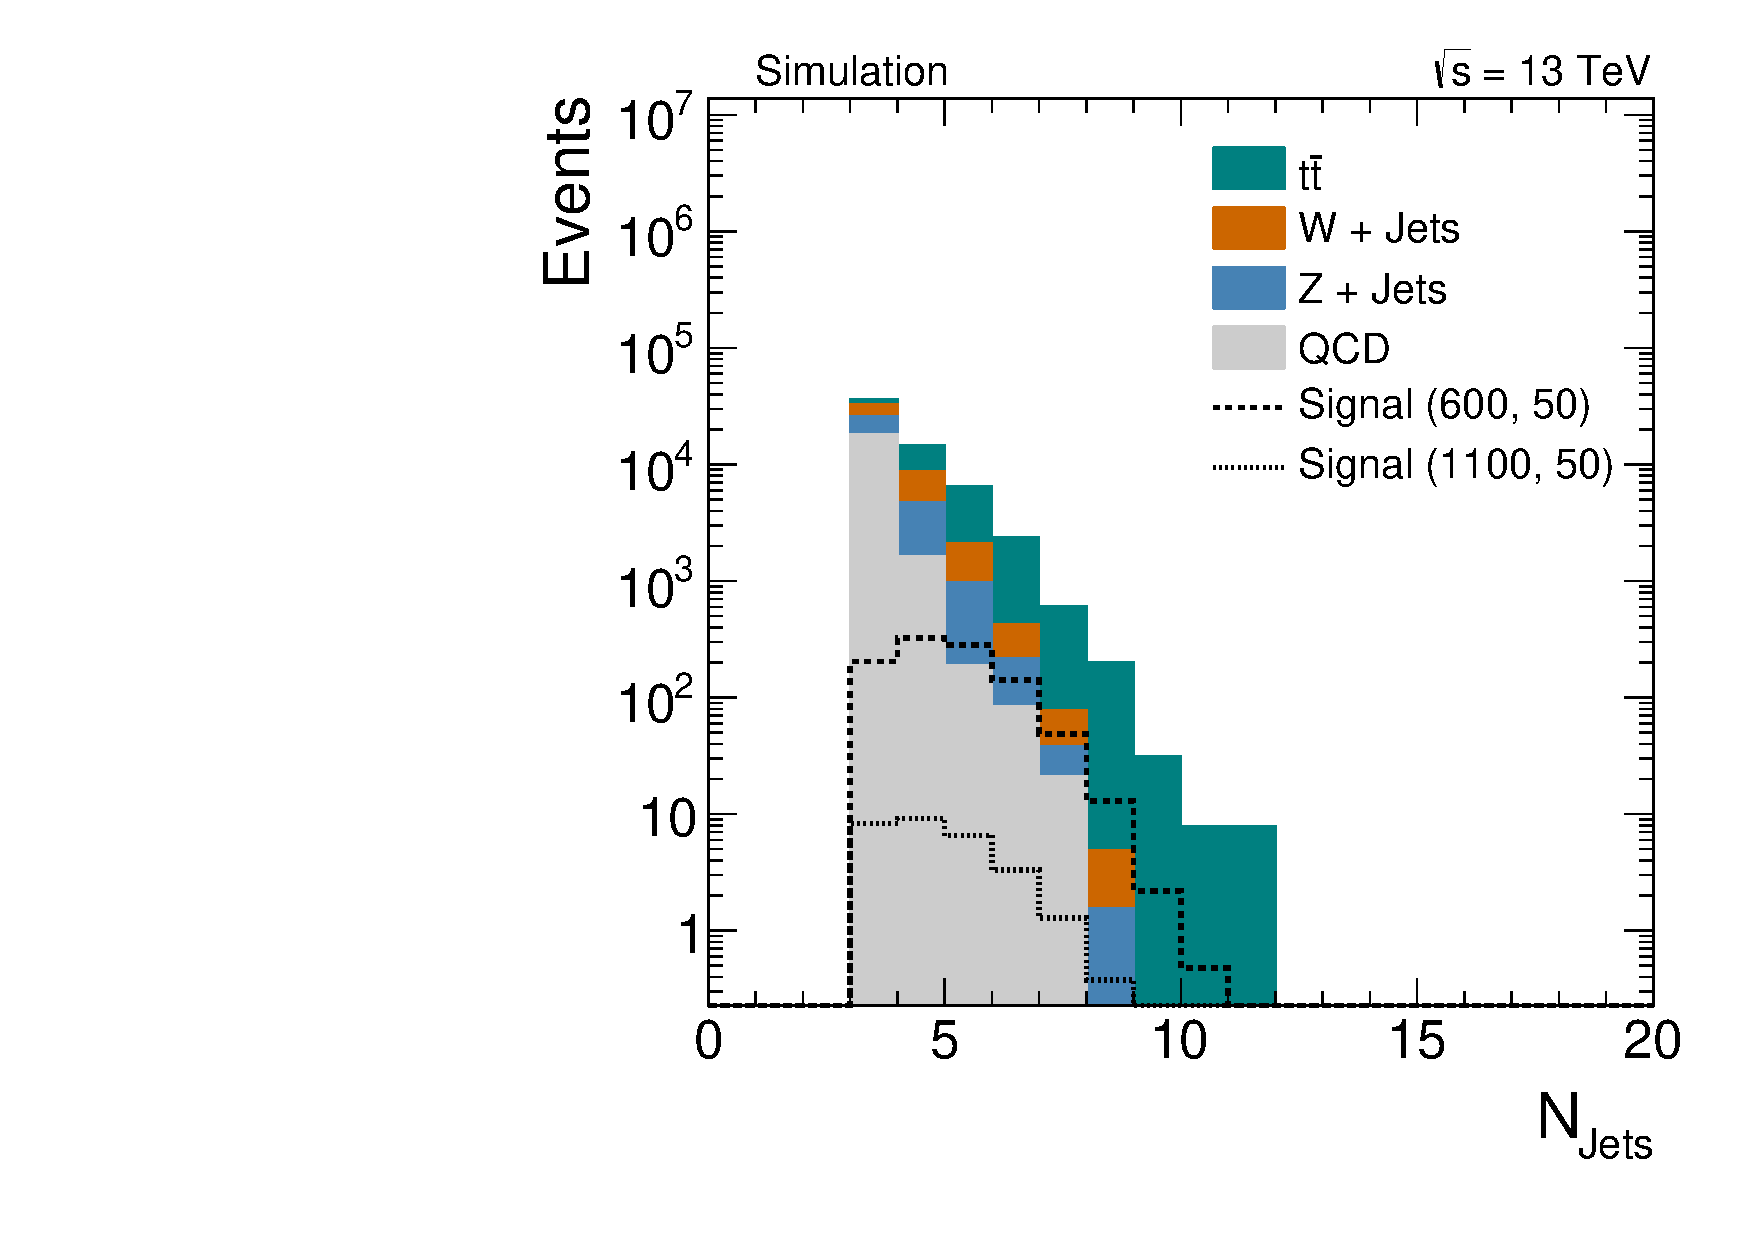
\includegraphics[width=0.49\textwidth]{figures/Stop_DeltaPhiSelection_N_jets.pdf}
    \end{center}
  \end{minipage}

  \caption{Comparison of selected \HT (\textit{top left}), \met (\textit{top right}) and \NJets (\textit{bottom}) distributions in simulated events found from applying the baseline selection criteria. The signal points are labeled as (X, Y) where X is the top squark mass and Y is the LSP mass.}
  \label{fig:stop_baseline}
\end{figure}
In order to investigate how this baseline selection can be further improved to gain sensitivity to the model of interest the evolution of the signal and background efficiencies is studied when changing specific selections in the analysis. In general, the signal and background efficiencies $\epsilon_\mathrm{sig/bg}$ are defined according to
\begin{equation}
\epsilon = \frac{\mathrm{no. \; of \; selected \; events}}{\mathrm{no. \; of \; all \; events}}
\end{equation} 

\begin{figure}[!t]
  \centering
\makebox[\linewidth]{
  \begin{tabular}{cc}
                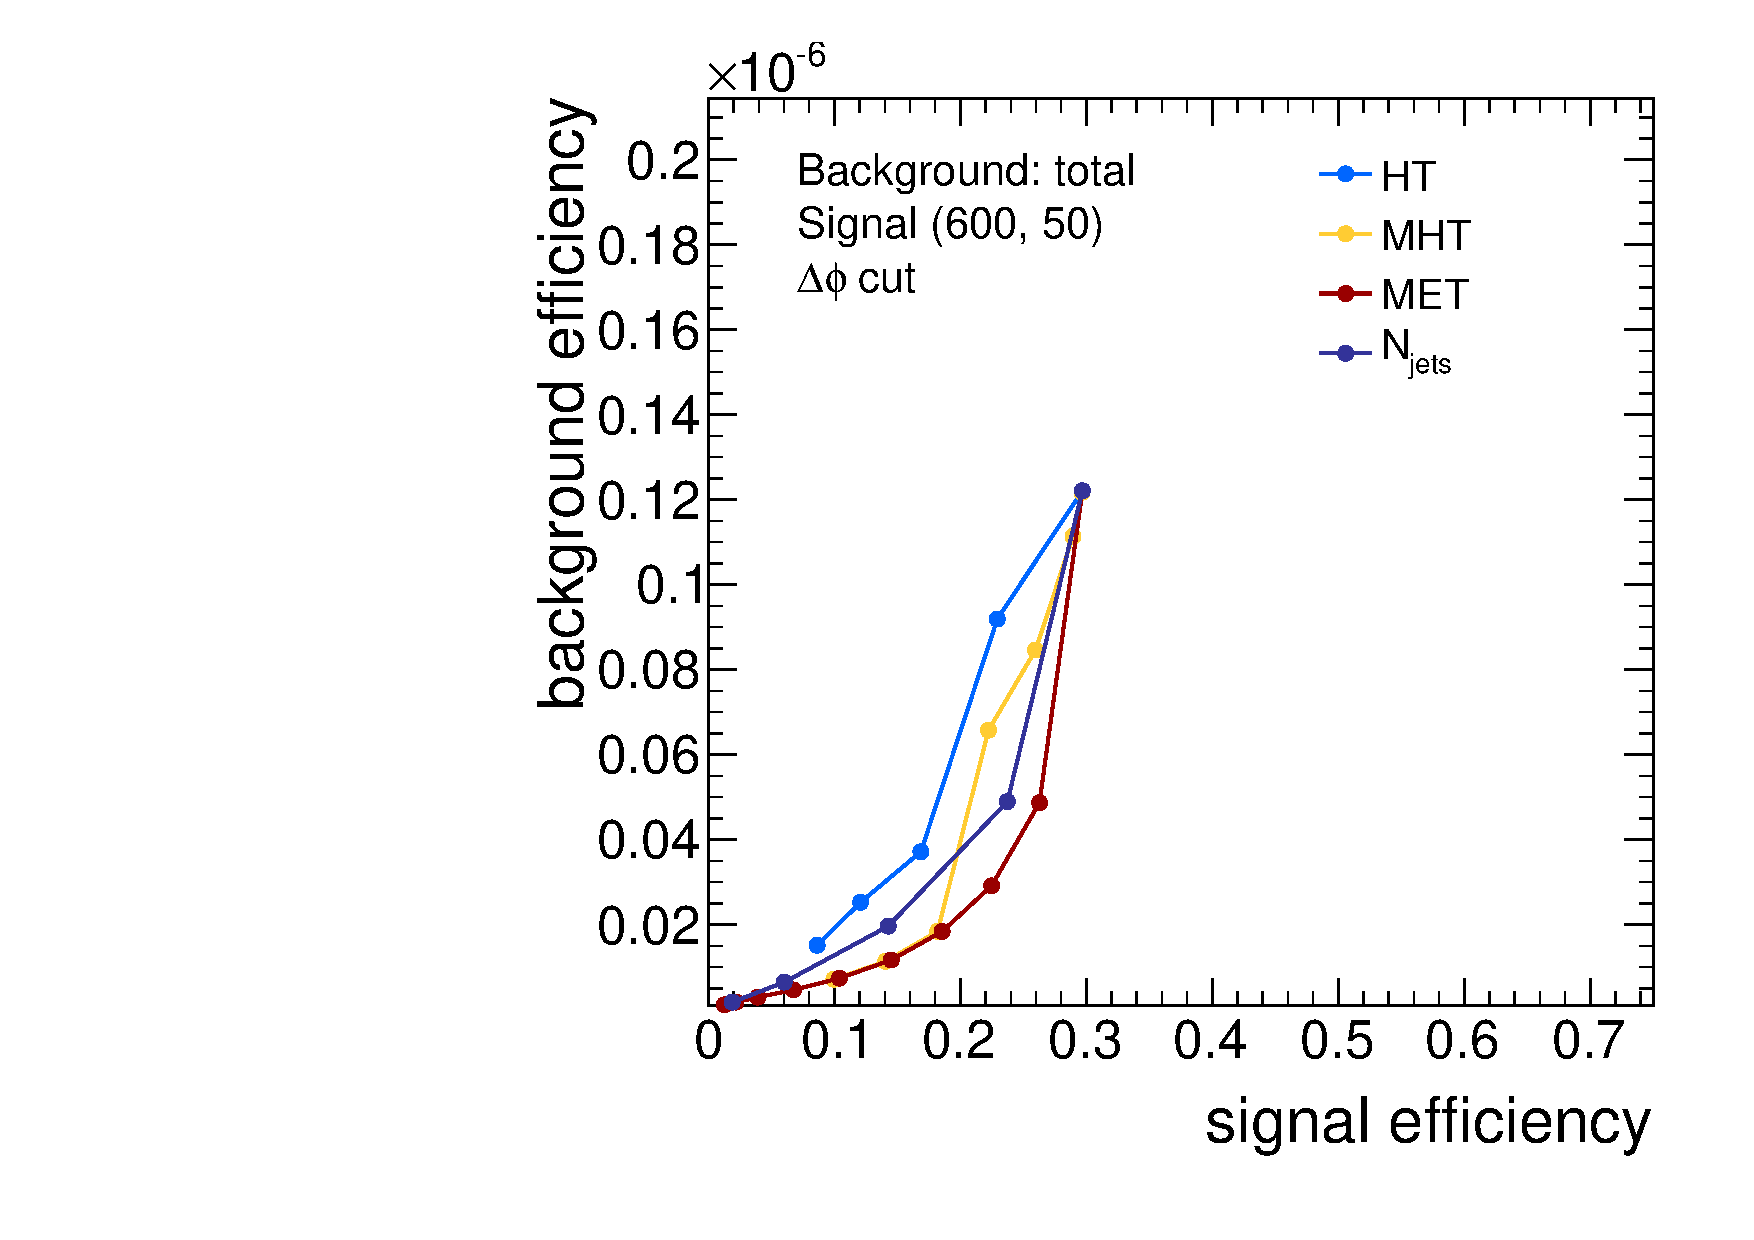
\includegraphics[width=0.49\textwidth]{figures/CutScan_DeltaPhiSelection_total_Stop600_LSP50_T2tt_13TeV_HT_MET_MHT_NJets.pdf} & 
                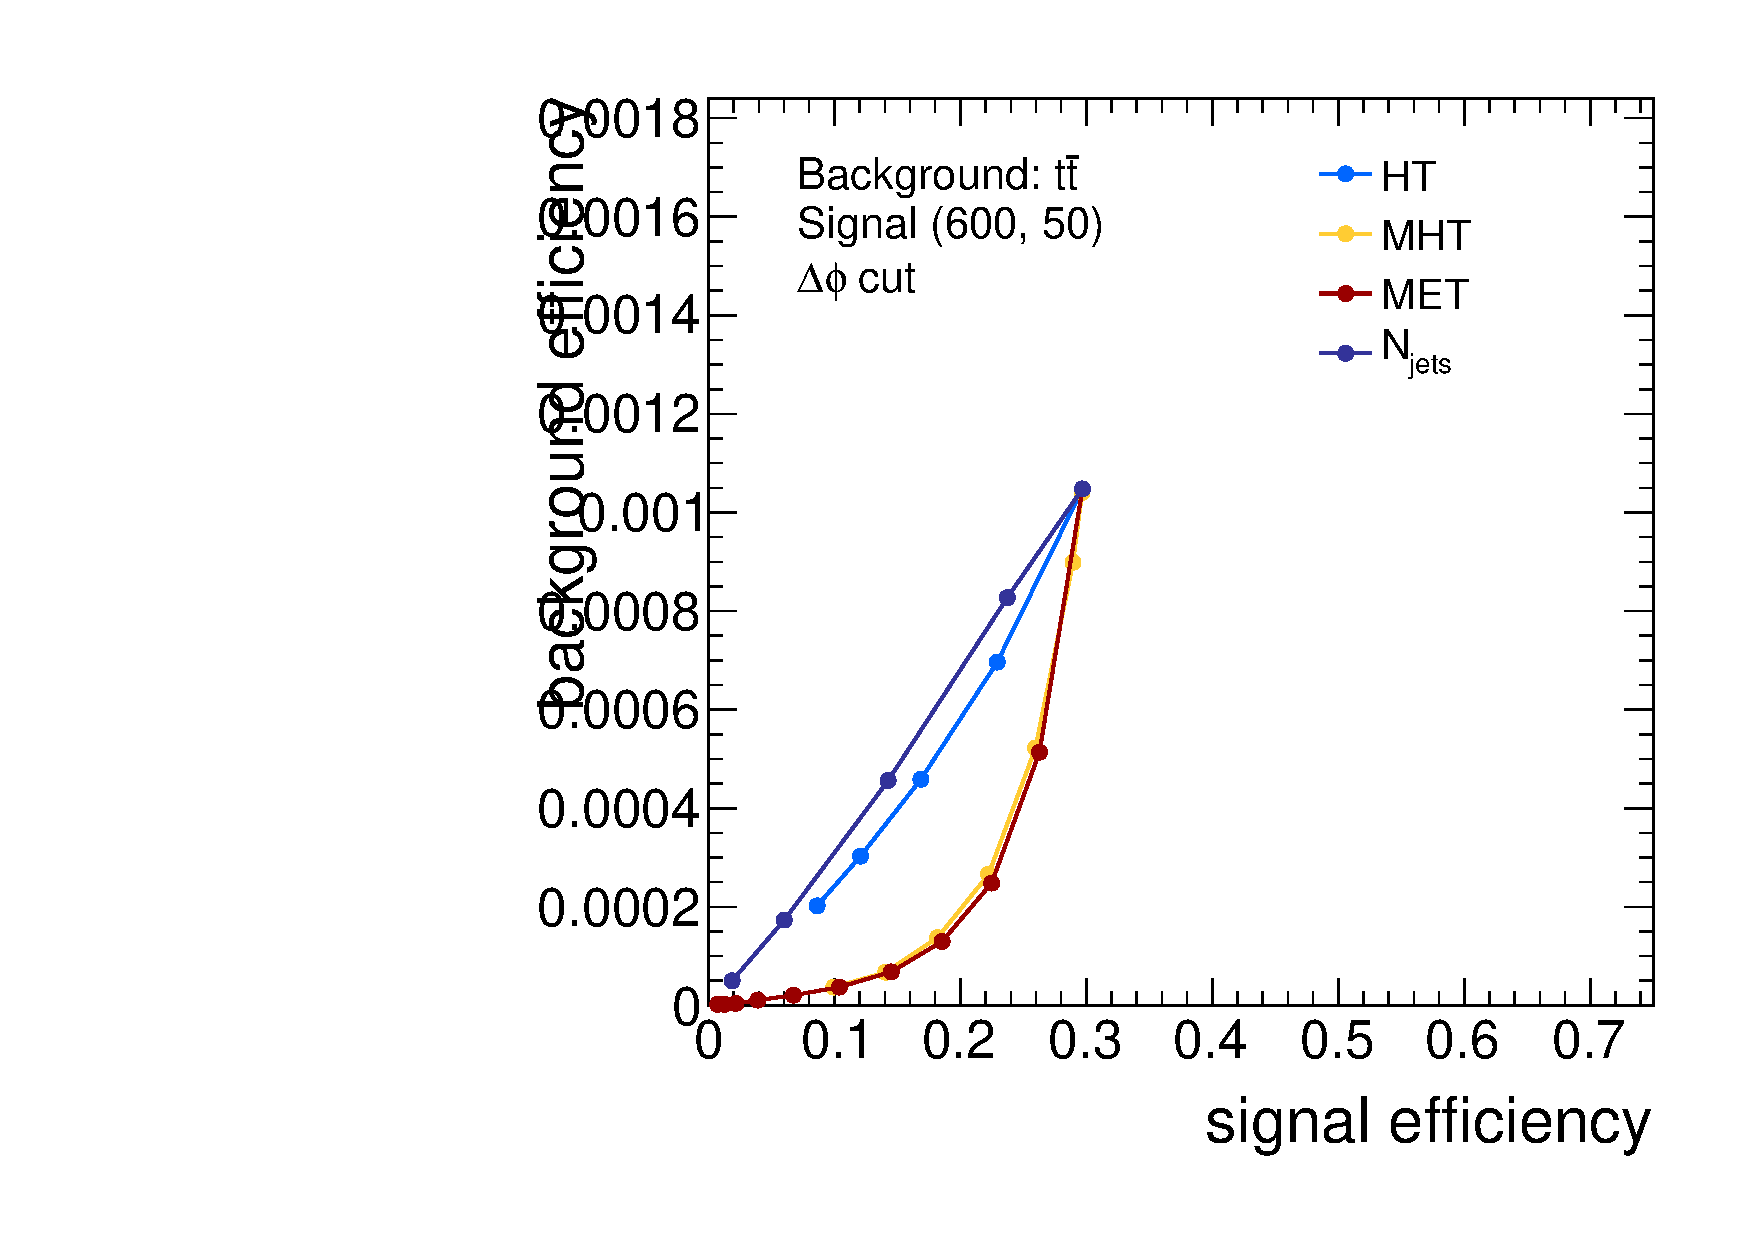
\includegraphics[width=0.49\textwidth]{figures/CutScan_DeltaPhiSelection_TTbar_powheg_13TeV_Stop600_LSP50_T2tt_13TeV_HT_MET_MHT_NJets.pdf} \\
                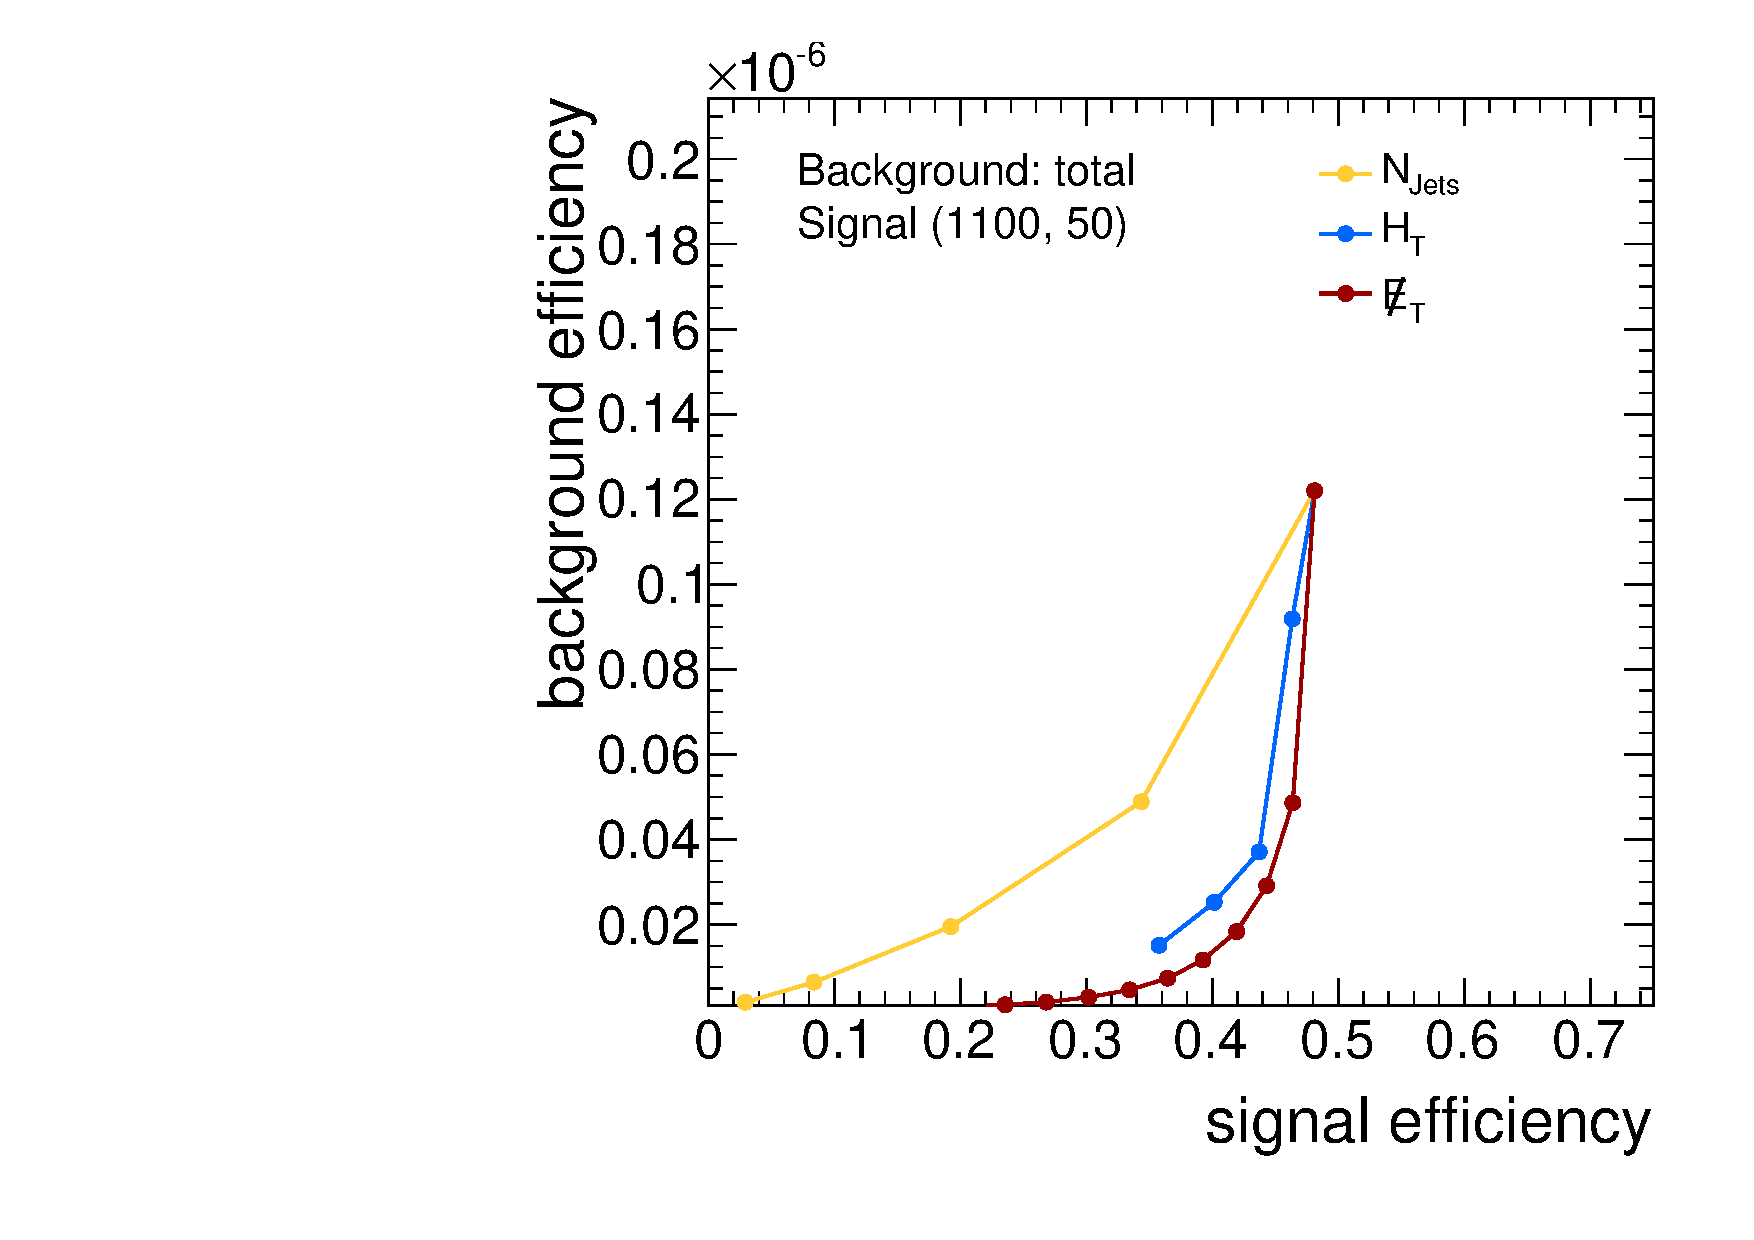
\includegraphics[width=0.49\textwidth]{figures/CutScan_DeltaPhiSelection_total_Stop1100_LSP50_T2tt_13TeV_HT_MET_MHT_NJets.pdf} &
                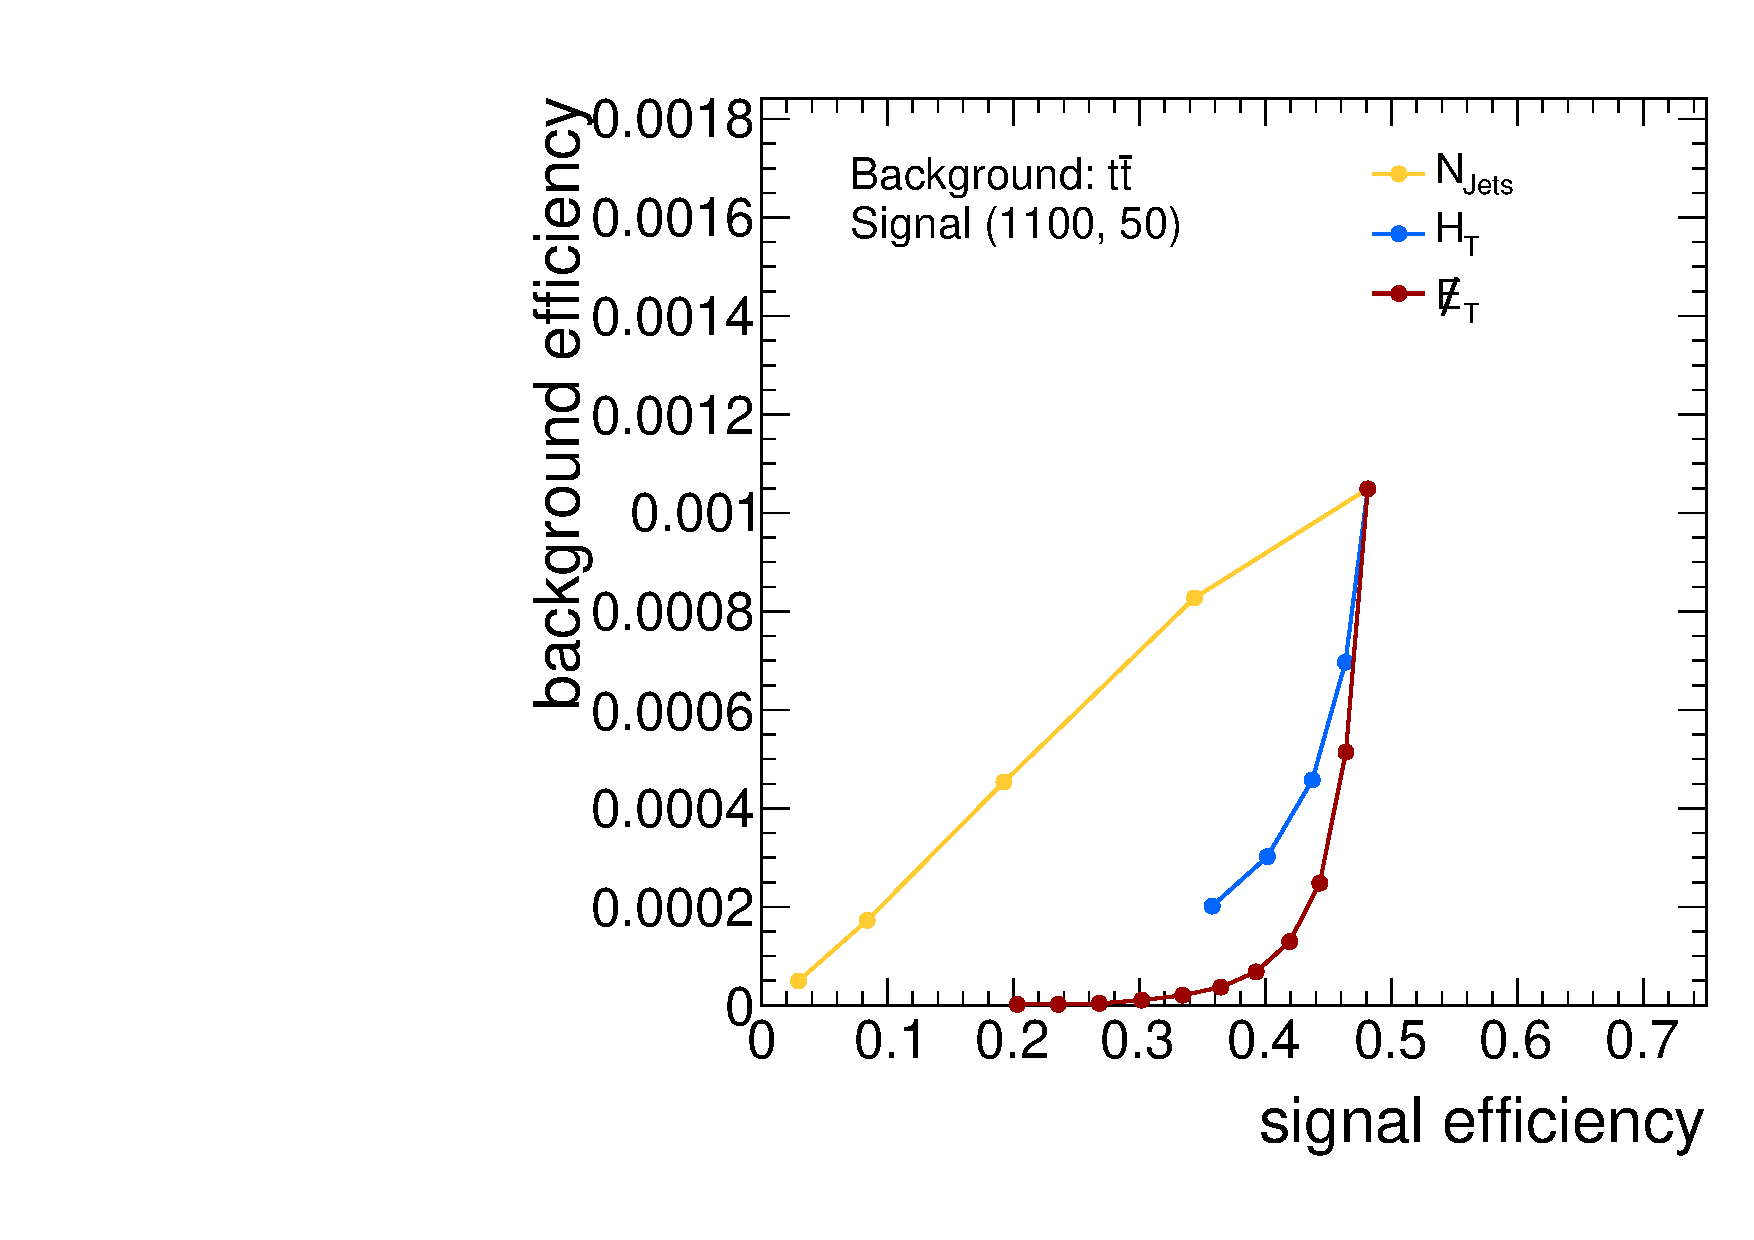
\includegraphics[width=0.49\textwidth]{figures/CutScan_DeltaPhiSelection_TTbar_powheg_13TeV_Stop1100_LSP50_T2tt_13TeV_HT_MET_MHT_NJets.pdf}
  \end{tabular}}
  \caption{Evolution of the signal versus background efficiency for a stop mass of 600\gev (\textit{top}) and 1100\gev (\textit{bottom}) where the background is the sum of all backgrounds (\textit{left}) or the \ttbar background (\textit{right}).}
  \label{fig:stop_baseline_cutscan_ht_met_mht_njets}
\end{figure}

for the number of signal and background events, respectively. In Fig.~\ref{fig:stop_baseline_cutscan_ht_met_mht_njets} the development of the signal versus background efficiencies are shown for the stop mass 600\gev and 1100\gev signal points and \ttbar as well as the total background events. The curves are obtained from increasing the cut value for the denoted variable by keeping the selection for all other variables fixed. The curve of a variable with good separation power runs close to the lower right corner. Here, the performance of \HT, \met and \NJets is compared. In addition to \met, also \MHT, as defined in Sec.~\ref{subsec:RA2_baseline}, is shown in this comparison. Both variables show a very similar performance such that in principle both variables could be employed with similar results. However, the performance of \met seems to be slightly better and thus this variable is used in these studies rather than \MHT. Furthermore, as stated above the same trigger as for the analysis presented in Chapter~\ref{chap:RA2} could be used to collect the data. Since this trigger is based on \met, the choice of the offline selections is closer to the online definition when using \met instead of \MHT. As can be seen in Fig.~\ref{fig:stop_baseline_cutscan_ht_met_mht_njets}, \met shows in general the best performance when comparing these variables. Furthermore, also \HT provides a good separation power and is only in case of the stop mass of 600~\gev inferior to \NJets. However, when only \ttbar background is considered, the jet multiplicity is not suitable as discriminating variable since the \NJets spectra of signal and \ttbar background are almost identical. As in general the kinematic features of \ttbar background are closest to the signal, it is of special importance to identify selections that can reduce this background. Consequently, \met and \HT are the preferred variables to distinguish signal and background processes. In the following, an analysis strategy close to the one described in Chapter~\ref{chap:RA2} is pursued. Events selected with the baseline selection are further categorized according to their \HT and \met values in exclusive search regions shown in Tab.~\ref{tab:stop_excl_search_bins}. \\ 
In order to determine the expected exclusion reach, the uncertainties for the individual background processes have to be considered. These are chosen in correspondence to the uncertainties obtained for similar kinematic regimes in the published all-hadronic stop analysis~\cite{CMS-PAS-SUS-13-015}. The respective uncertainties considered for the different processes are
\begin{itemize}
 \item QCD multijet events: 100\%
 \item \ZJets: 50\%
 \item \WJets: 20\%
 \item \ttbar: 20\% + additional 20\% in the high \met search regions
\end{itemize}  
which are meant to be total uncertainties such that the actual statistical uncertainty of the number of simulated MC events is not considered explicitly. Based on the selected event yields and the estimated uncertainties the 95\% confidence-level expected upper limit is calculated as an asymptotic $\mathrm{CL_s}$ limit~\cite{bib:theta}. The obtained exclusion curve is shown in Fig.~\ref{fig:stop_baseline_limit} for the signal strength $\mu$ which is the excluded production cross section divided by the theoretical cross section for direct stop production as function of the stop quark mass. Consequently, a particular mass point can be excluded, if the expected limit drops below one. However, it turns out that this baseline selection cuts and the subsequent binning in exclusive search regions is not yet sensitive enough to probe any of the selected mass points. Thus, possible improvements of the analysis are discussed in the following sections.  

\begin{table}[!t]
%\fontsize{10 pt}{1.2 em}
%\selectfont
\centering
\caption{Exclusive search regions used in the analysis binned in \HT and \met.}
\begin{tabular}{l|c}
\multicolumn{2}{c}{} \\
  \toprule
               & \met [\gev]    \\
  \midrule
   \HT $= 500 - 1000$\gev  & 200 - 400  \\
                          & $>$ 400  \\
  \midrule
   \HT $>$ 1000\gev  & 200 - 400  \\
                 & $>$ 400  \\
                   
  \bottomrule
\end{tabular}
\label{tab:stop_excl_search_bins}
\end{table}    


\begin{figure}[!h]
  \centering
  \begin{tabular}{c}
                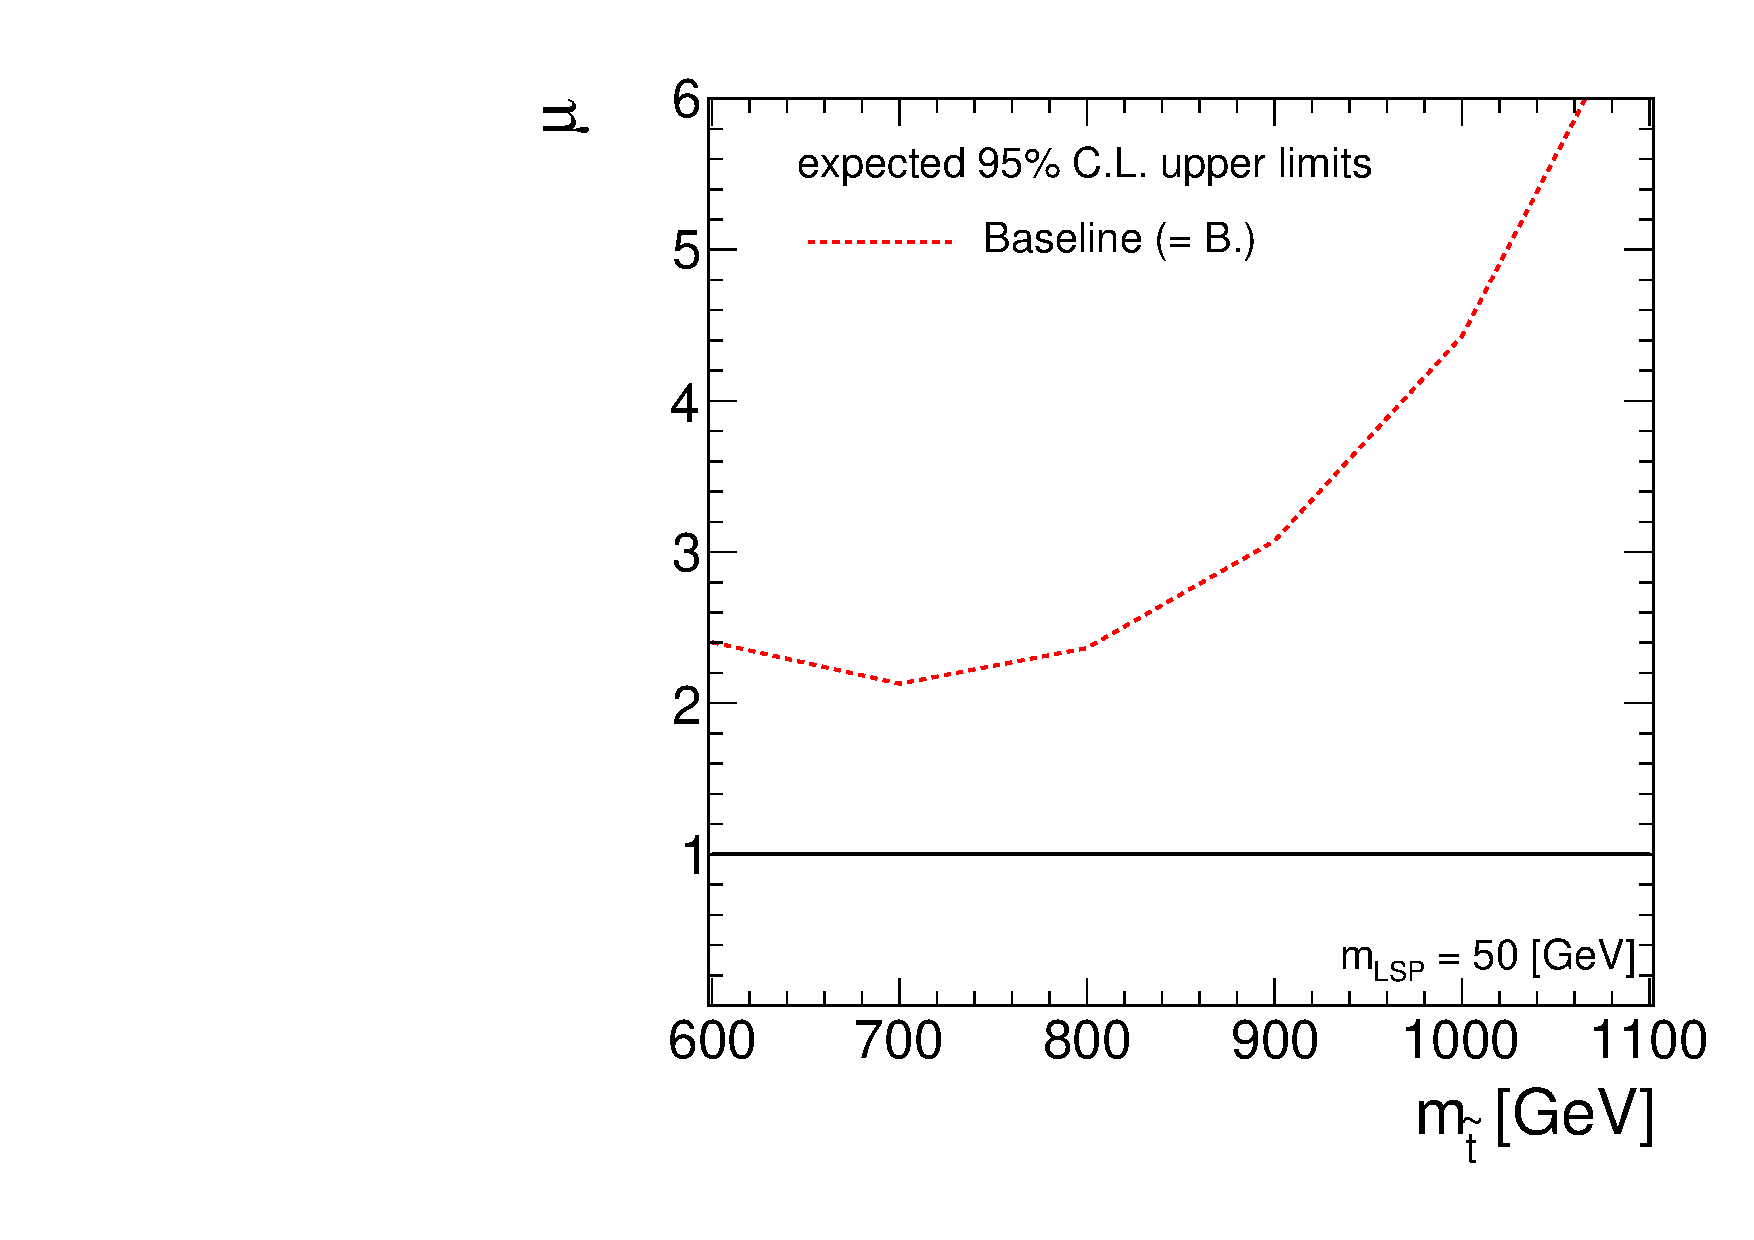
\includegraphics[width=0.75\textwidth]{figures/limitplot4BinSel_Baseline.pdf} 
  \end{tabular}
  \caption{Expected 95\% upper limit for signal strength versus $m_{\tilde{t}}$. The LSP mass is chosen to be 50\gev.}
  \label{fig:stop_baseline_limit}
\end{figure}

\section{Sensitivity Improvement using b Tagging}
\label{sec:stop_btagging}
As illustrated in Fig.~\ref{fig:T2tt}, the targeted signal final state involves the presence of bottom quarks emerging from the decay of the top quarks. Thus, a very common thing to possibly enhance the sensitivity of such an analysis is to employ b-tagging techniques to identify the b quarks in the final state. Typical b-tagging algorithms for the identification of b-quark jets used within the CMS experiment have been discussed in Section~\ref{sec:btagging}. In this analysis b-quark jets are identified based on the CSV-algorithm using the medium working point. In Fig.~\ref{fig:stop_baseline_btag} the b-tag multiplicity, \ie the number of b-tagged jets in the event is illustrated. As expected the maximum of this distribution for signal and \ttbar events is around two, since two b-quark jets are expected from the two decaying top quarks. Values above two or b-tagged jets in backgrounds not containing real b-quarks can be explained by the misidentification rate of the tagging algorithm. \\
The resulting distributions for \HT, \met and \NJets after requiring the presence of at least one b-tagged jet in the event are illustrated in Fig.~\ref{fig:stop_baseline_btag_HT_MET_NJets}. It can be seen that all backgrounds except for \ttbar can be significantly reduced when requiring the presence of at least one b-quark jet. \\
\begin{figure}[!t]
  \centering
  \begin{tabular}{c}
                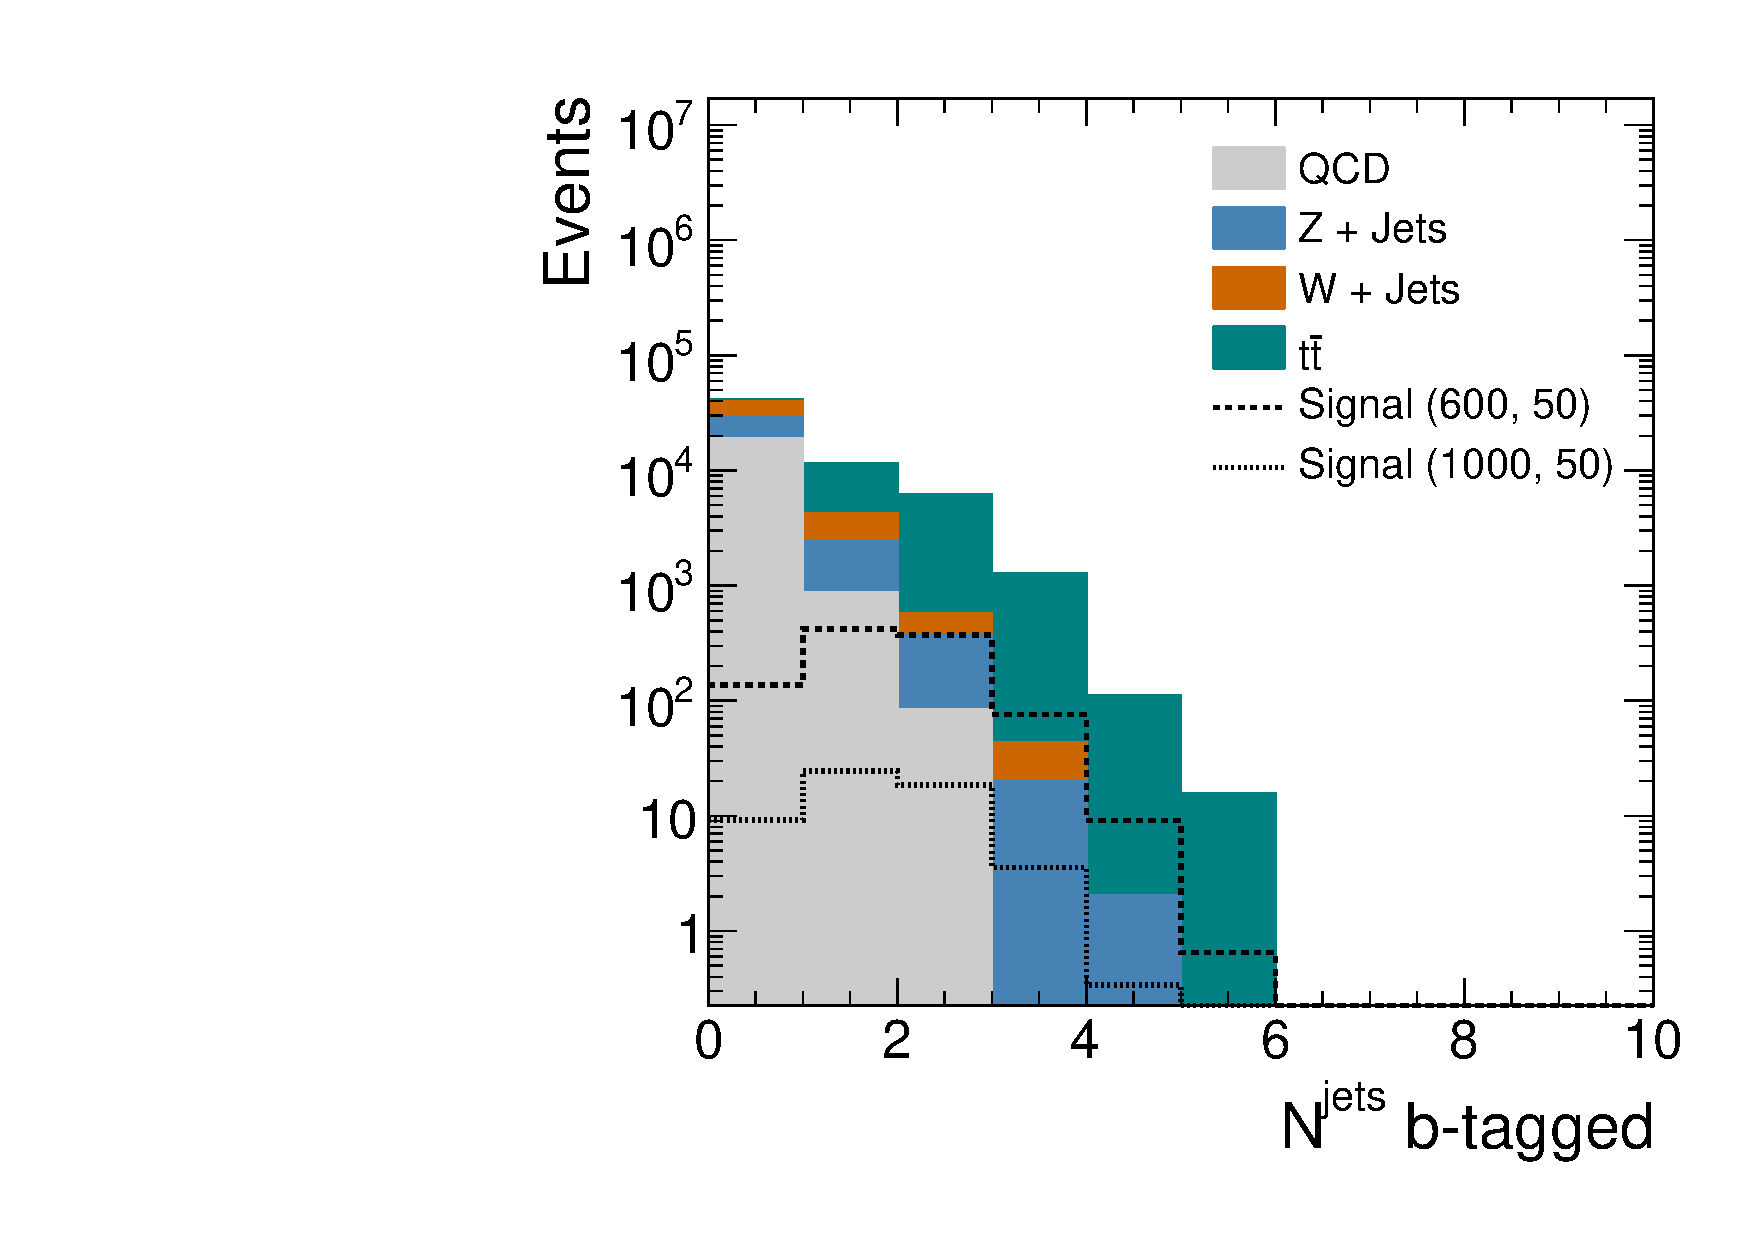
\includegraphics[width=0.49\textwidth]{figures/Stop_DeltaPhiSelection_N_jets_btagged.pdf} 
  \end{tabular}
  \caption{B-tag multiplicity after applying the baseline selection in simulated events. The signal points are labeled as (X, Y) where X is the top squark mass and Y is the LSP mass.}
  \label{fig:stop_baseline_btag}
\end{figure}
\begin{figure}[!t]
  \centering
  % \makebox[\linewidth]{
  \begin{minipage}[c]{1.\textwidth}
    \begin{center}
      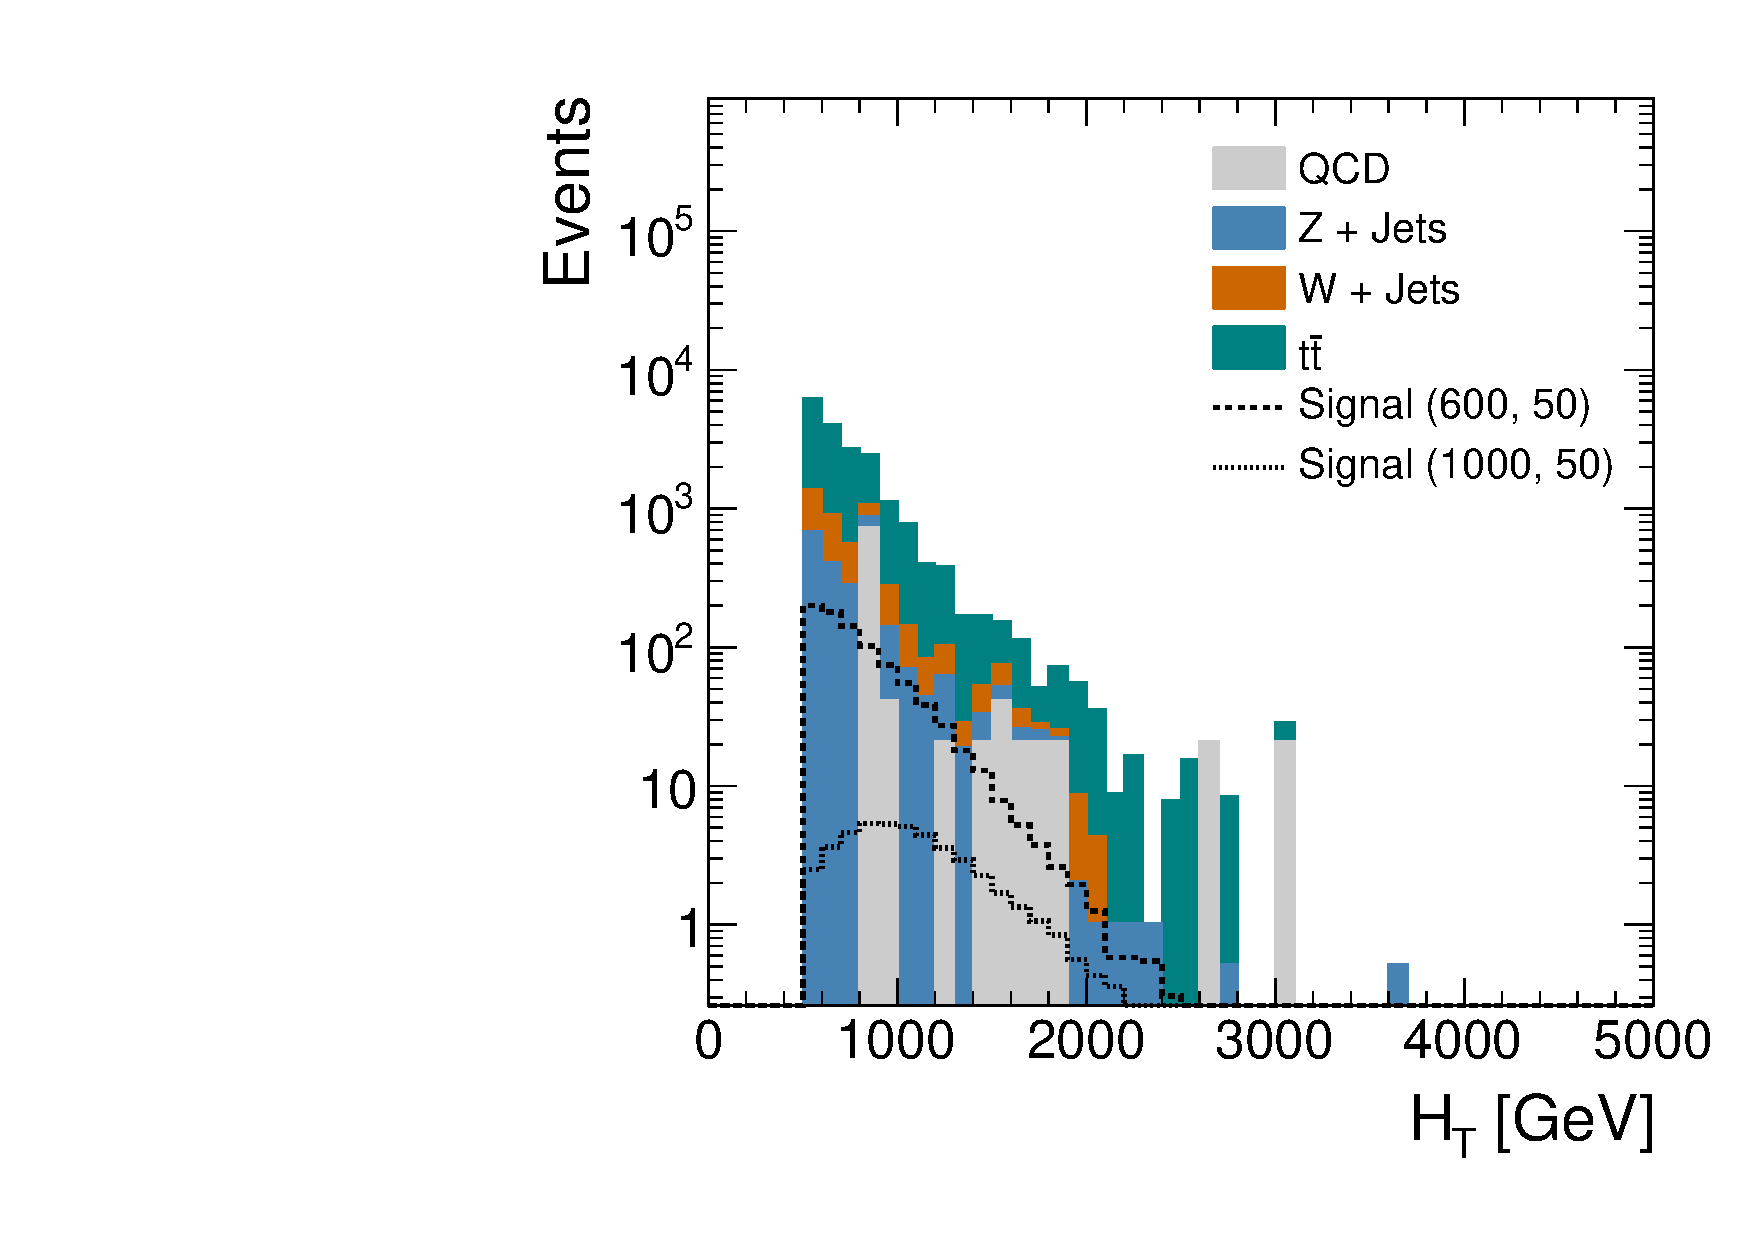
\includegraphics[width=0.49\textwidth]{figures/Stop_BTag_HThad.pdf}  
      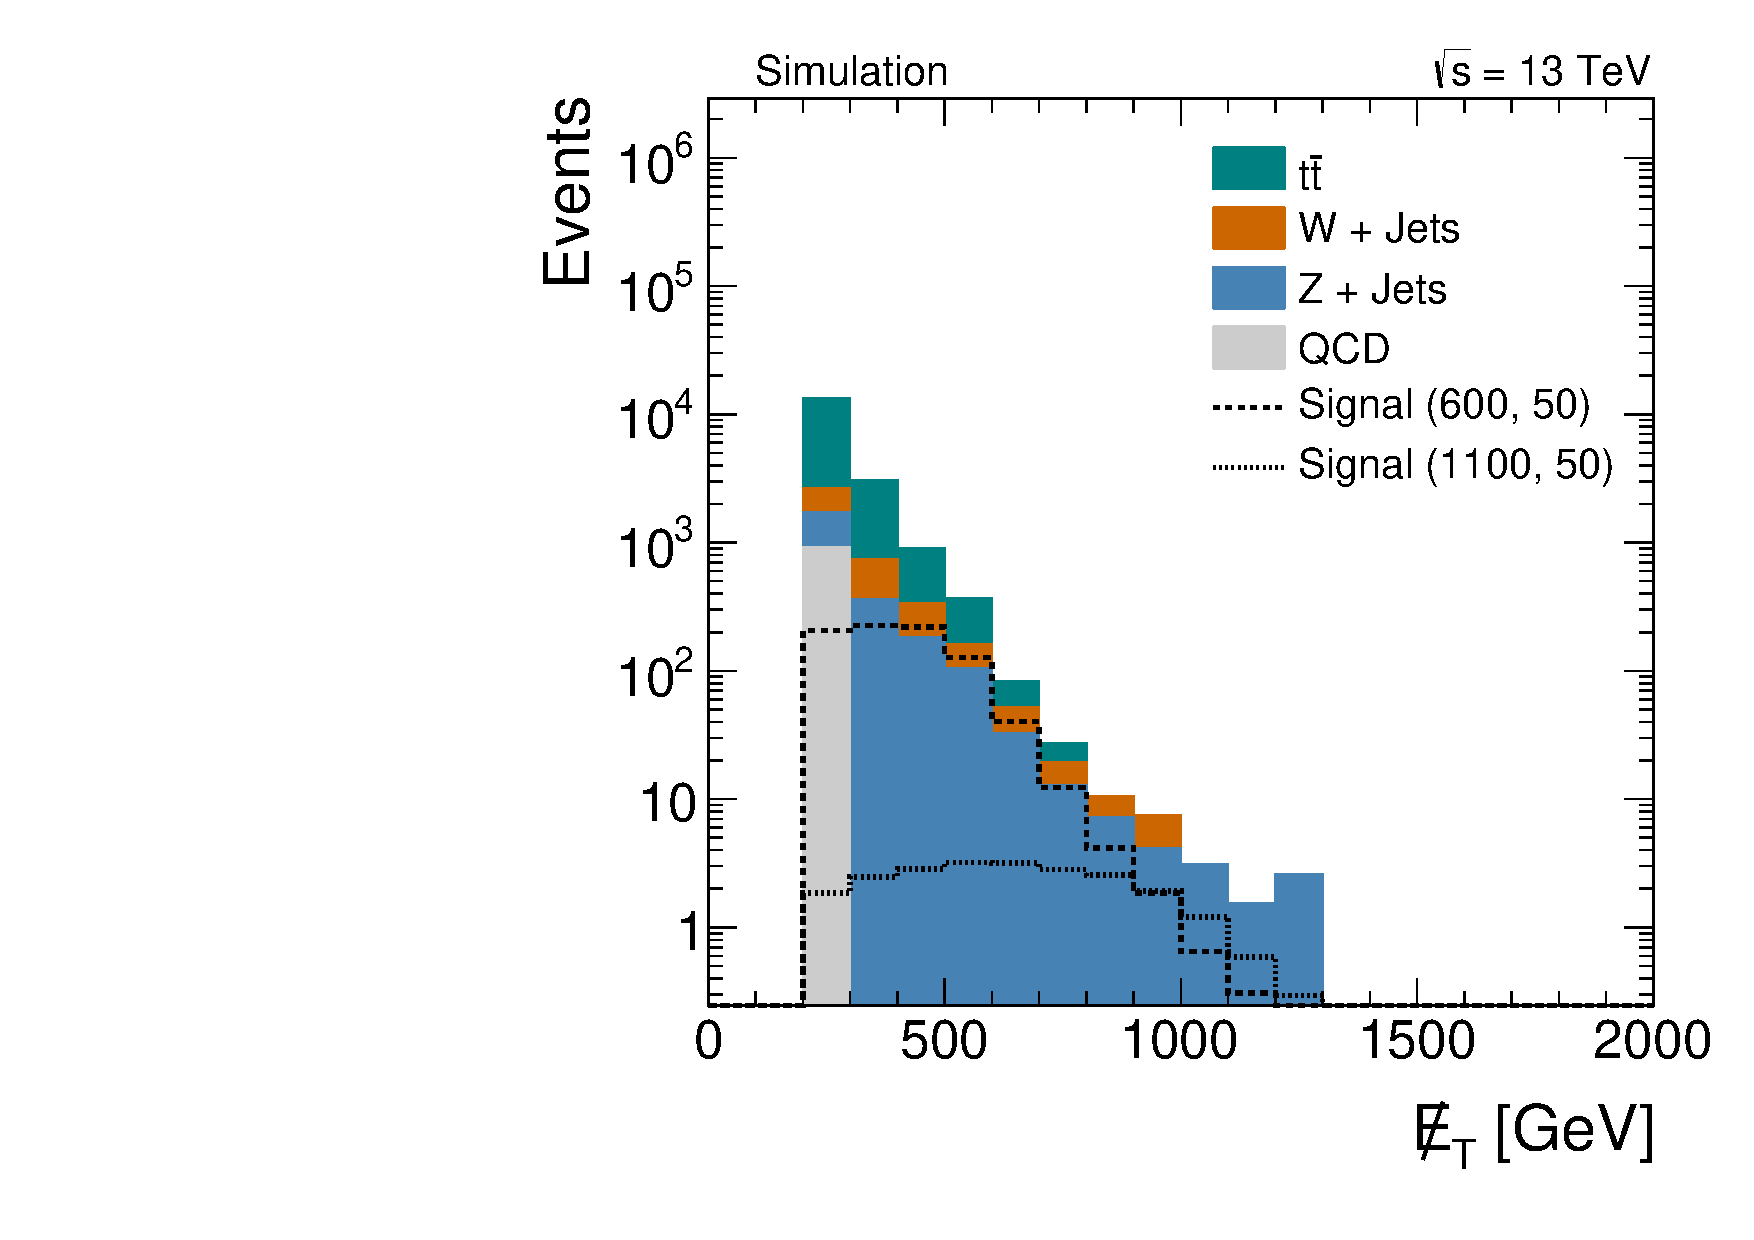
\includegraphics[width=0.49\textwidth]{figures/Stop_BTag_MET.pdf} \\
      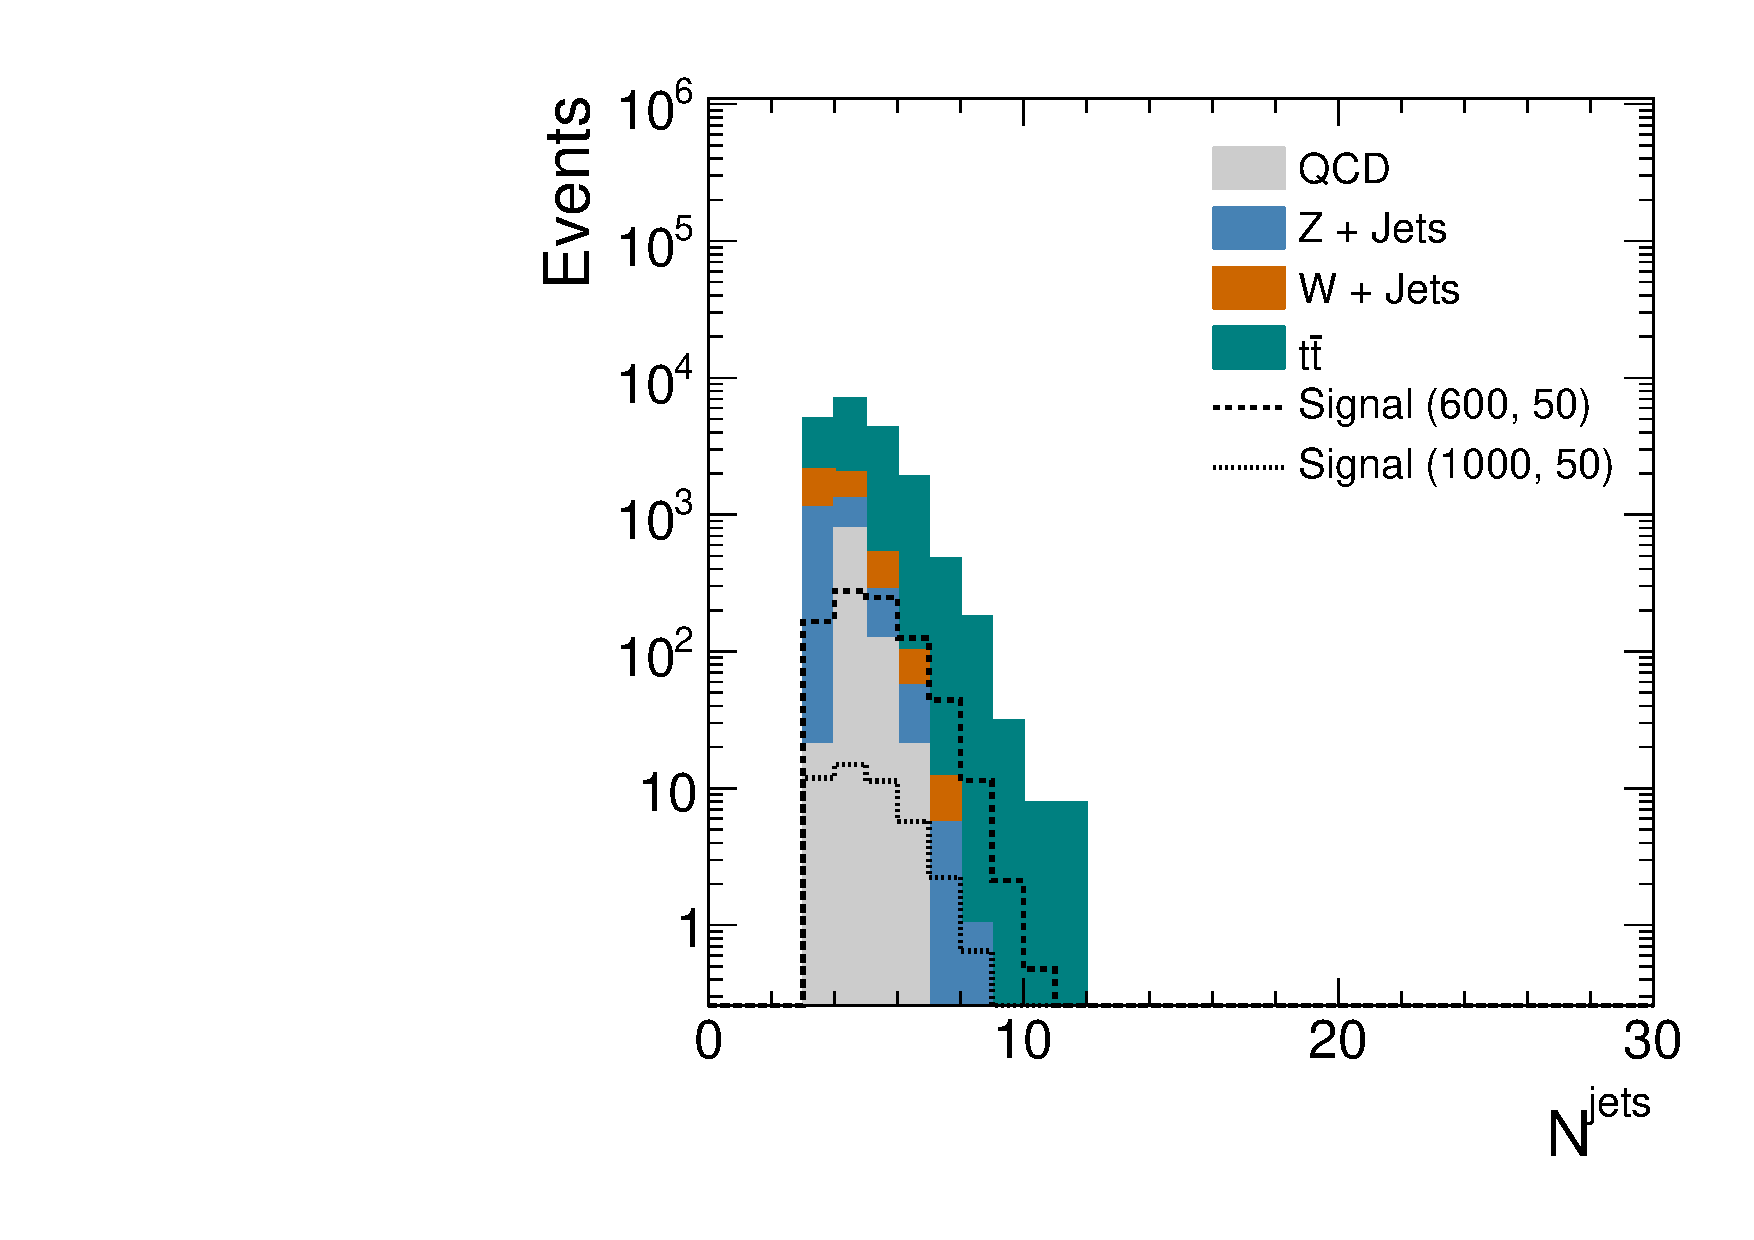
\includegraphics[width=0.49\textwidth]{figures/Stop_BTag_N_jets.pdf}
    \end{center}
  \end{minipage}

  \caption{Comparison of selected \HT (\textit{top left}), \met (\textit{top right}) and \NJets (\textit{bottom}) distributions in simulated events found from applying the baseline selection criteria and requiring at least one b-tagged jet. The signal points are labeled as (X, Y) where X is the top squark mass and Y is the LSP mass.}
  \label{fig:stop_baseline_btag_HT_MET_NJets}
\end{figure}
Consequently, the expected exclusion reach of the analysis is supposed to improve when applying the b-tag requirement in addition to the baseline selection. Thus, the same exclusive search regions as defined in Tab.~\ref{tab:stop_excl_search_bins} are used considering the same total uncertainties as described in Sec.~\ref{sec:stop_baseline} for a performance comparison of this improved selection with respect to the baseline requirements. The expected limits for the baseline selection as well as the baseline selection and the b-tag requirement are shown in Fig~\ref{fig:stop_baselinebtag_limit}. It turns out that the b-tag requirement significantly improves the sensitivity of the analysis towards the specified top squark mass range. Especially lower masses could be tested with such an anlaysis strategy. However, since the focus of this analysis is put on higher stop quark masses, it is discussed in the next section how this mass range can be adressed better.  

\begin{figure}[!h]
  \centering
  \begin{tabular}{c}
                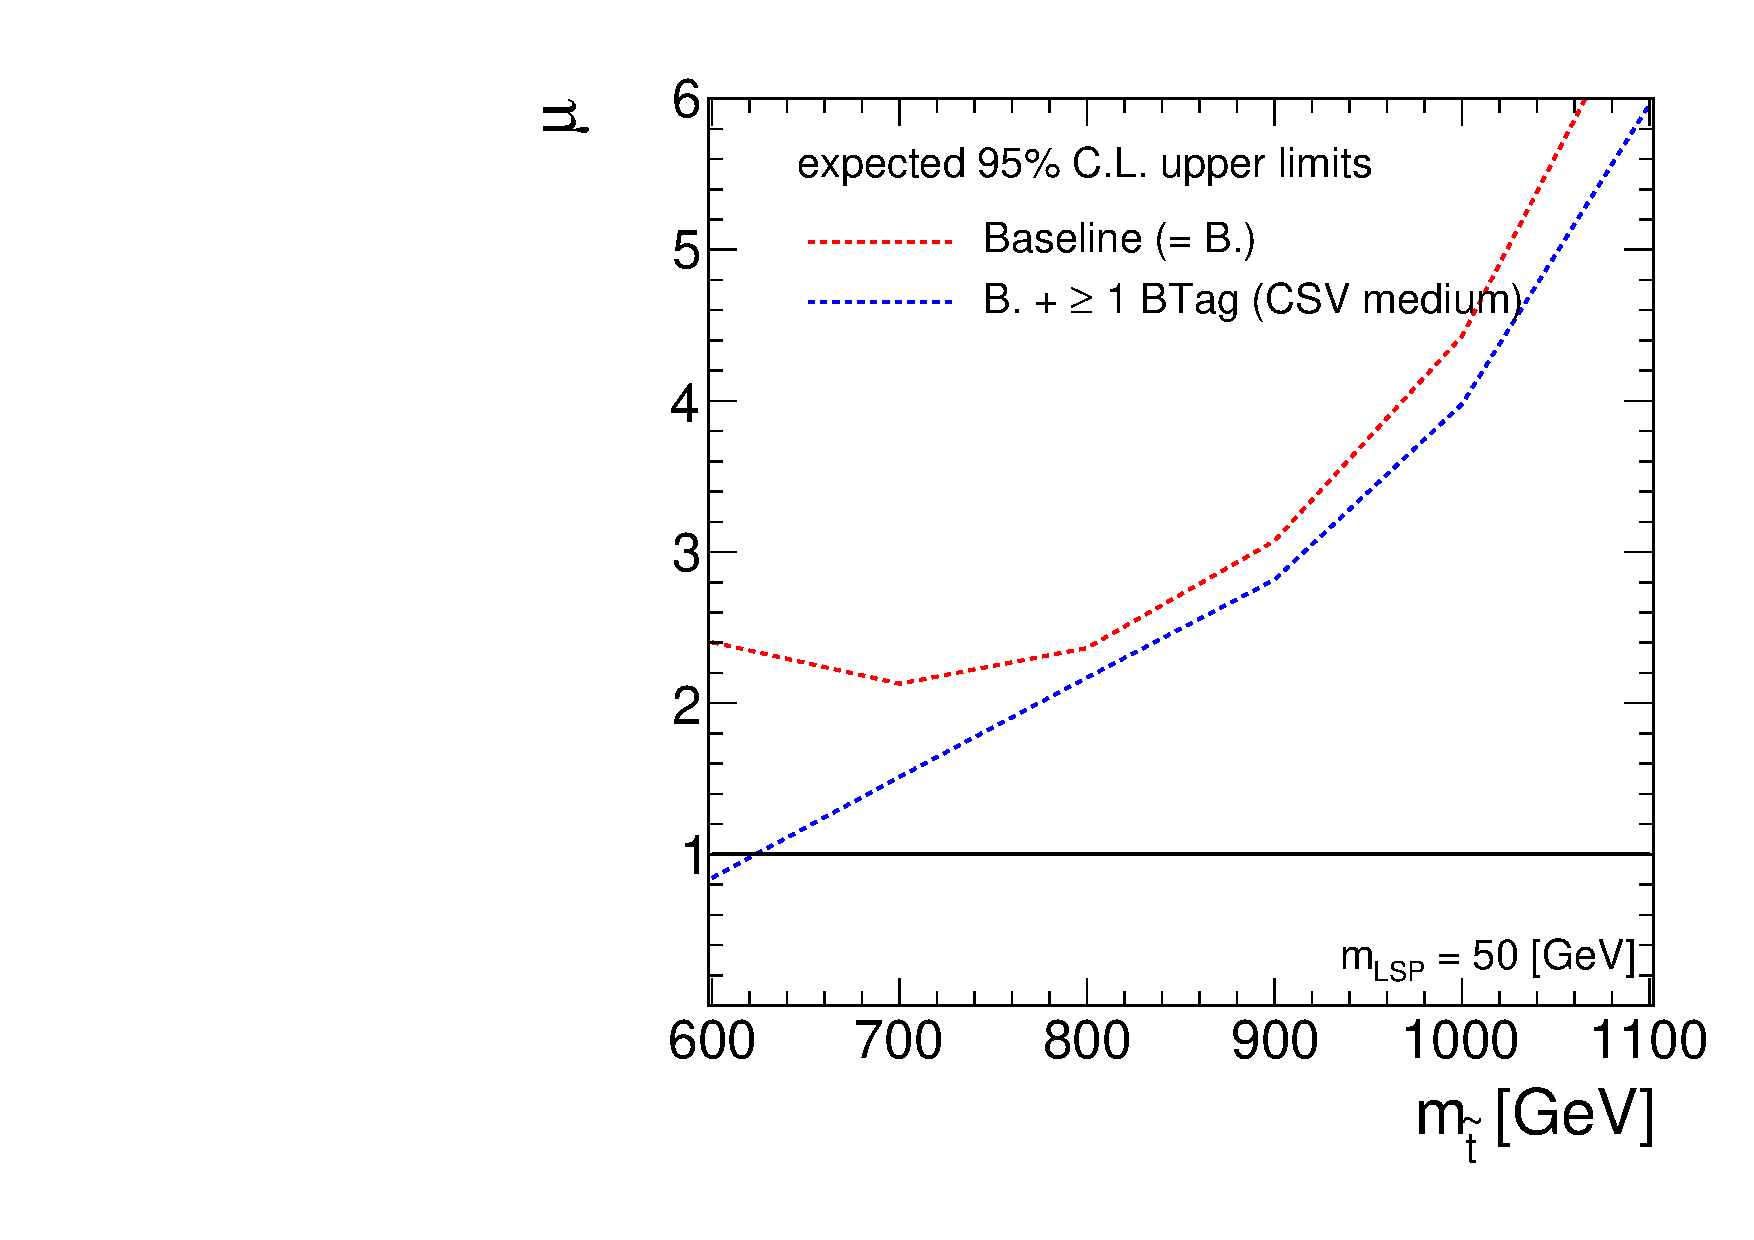
\includegraphics[width=0.75\textwidth]{figures/limitplot4BinSel_BaselineBTag.pdf} 
  \end{tabular}
  \caption{Expected 95\% upper limit for signal strength versus $m_{\tilde{t}}$. The LSP mass is chosen to be 50\gev.}
  \label{fig:stop_baselinebtag_limit}
\end{figure}

\section{Sensitivity Improvement using top Tagging}
\label{sec:stop_btagging}

\subsection{Top Tagging Efficiency Studies}
\label{subsec:stop_toptagging}

\begin{description}
 \item \textbf{Top Tag Efficiency}
 \item \textbf{Misidentification Rate}
\end{description}

\begin{figure}[!h]
  \centering
  \begin{tabular}{c}
                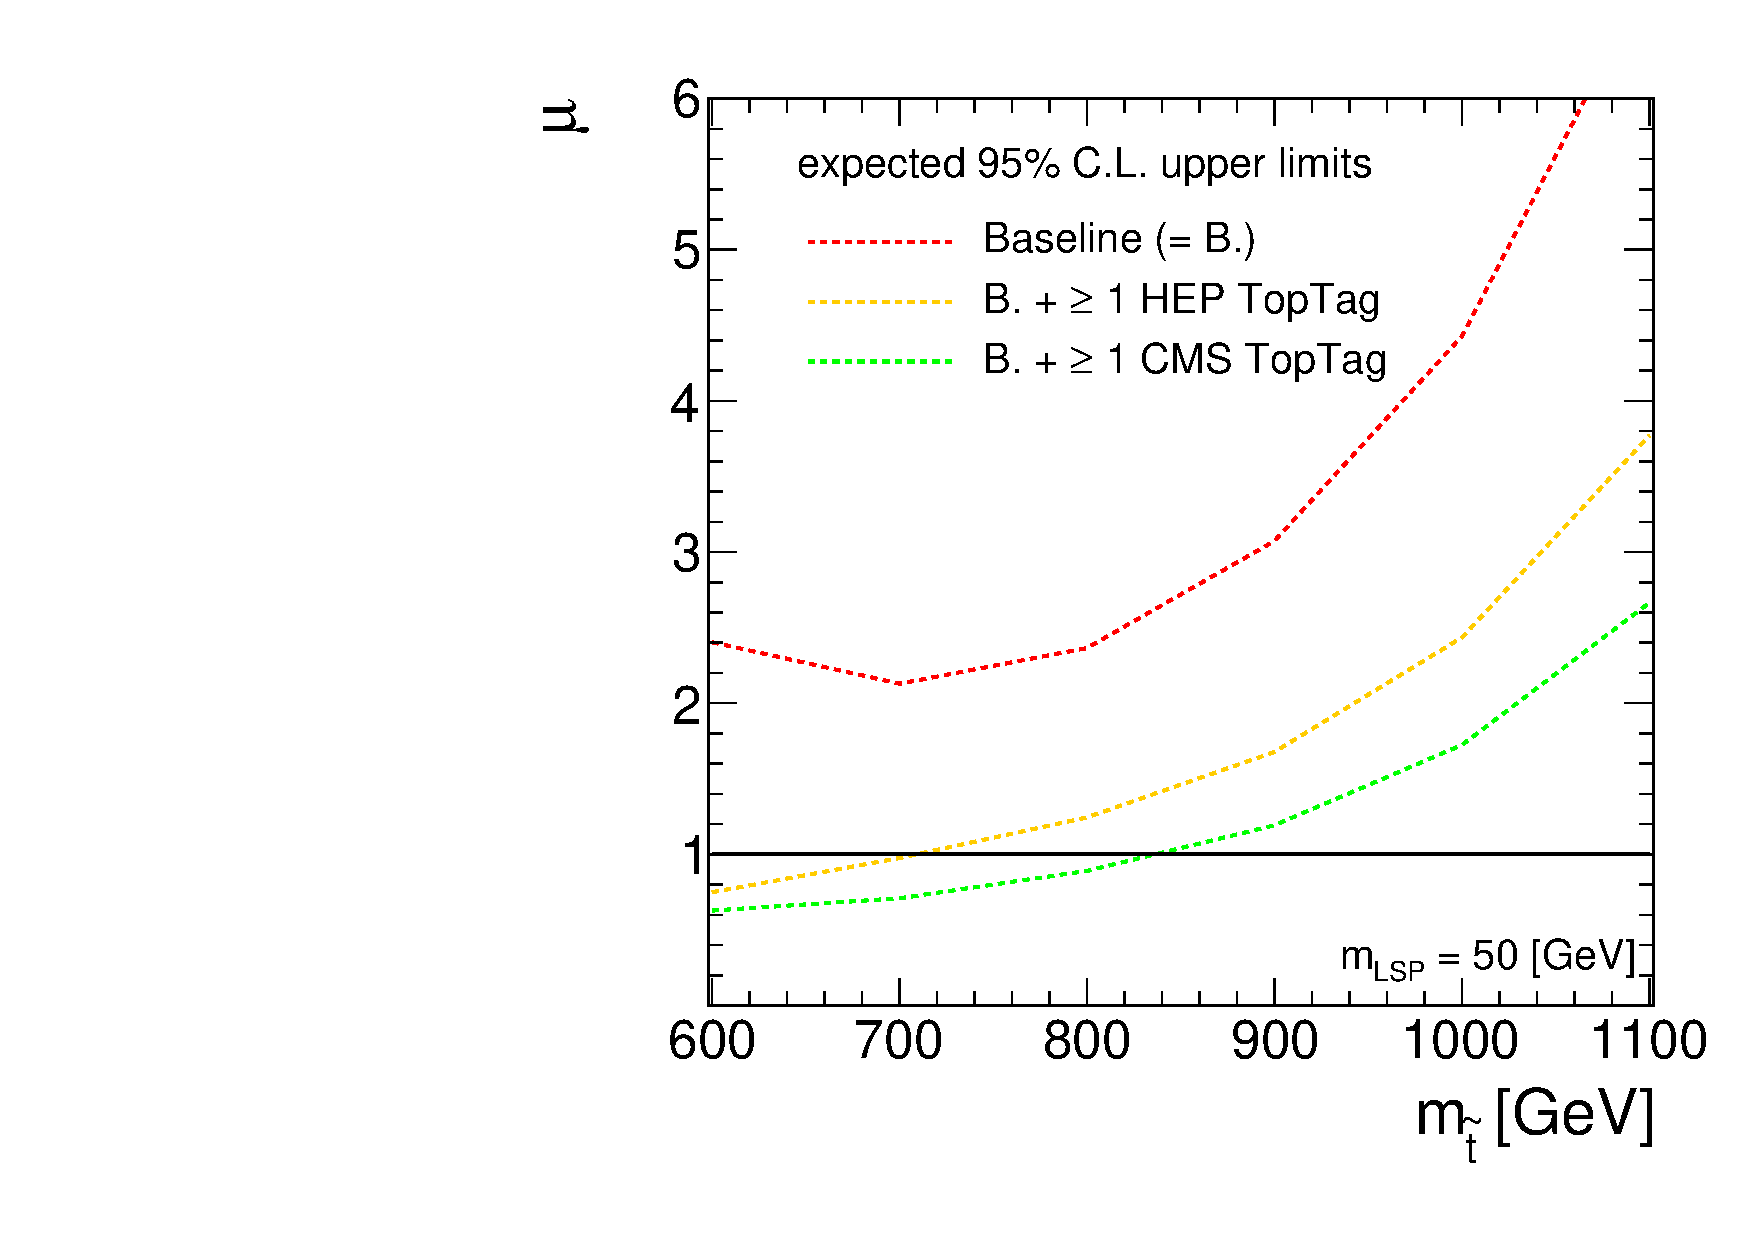
\includegraphics[width=0.75\textwidth]{figures/limitplot4BinSel_BaselineTopTag.pdf} 
  \end{tabular}
  \caption{Expected 95\% upper limit for signal strength versus $m_{\tilde{t}}$. The LSP mass is chosen to be 50\gev.}
  \label{fig:stop_baselinetoptag_limit}
\end{figure}

\section{Performance Comparison of Various Kinematic Selections}
\label{sec:stop_cuts}

\section{Performance Comparison to Published Analysis}
\label{sec:stop_pub}

\section{Studies of Alternative Selections}
\label{sec:stop_alternatives}

\section{Sensitivity to Gluino-Mediated Stop Production}
\label{sec:stop_gluinos}

\section{Results and Discussion}
\label{sec:stop_results}


